\subsection{微波} % (fold)
	\label{sub:微波}
	\subsubsection{微波的性质} % (fold)
		\label{ssub:微波的性质}
		\par 微波即波长范围在1mm-1m的电磁波的总称,对应频率为$3\times 10^{8\sim 11}$Hz。微波的振荡周期接近真空电子管中的电子渡越时间($\sim$10\textsuperscript{-10}s),使得电子在微波振荡中的滞后效应不可忽略;微波的波长与一般宏观物体(包括通常的电子元件)相当,因此会在宏观物体表面产生反射,并可由一般电子元件产生,且只能在波导管/谐振腔等中传输,而其电磁场参量在一般电路中需要用分布参数来描述;微波传播类似可见光,有直线传播/反射/吸收/折射等效应,而又可穿透电离层(区别于其它无线电波),常被用于卫星通信等领域,但借助微波的地面通讯则须借助中继站;微波量子能量许多原子/分子的振动-转动能级和磁能级相近,适用于相关研究。由于这些特性与其它波段电磁波都有不同,微波的产生/传播等都有专门的理论描述和技术实现。\supct{bib:textbook}
	% subsubsection 微波的性质 (end)
	\subsubsection{微波的产生} % (fold)
	\label{ssub:微波的产生}
		\FloatBarrier
		\begin{wrapfigure}[]{r}[0pt]{5cm}
			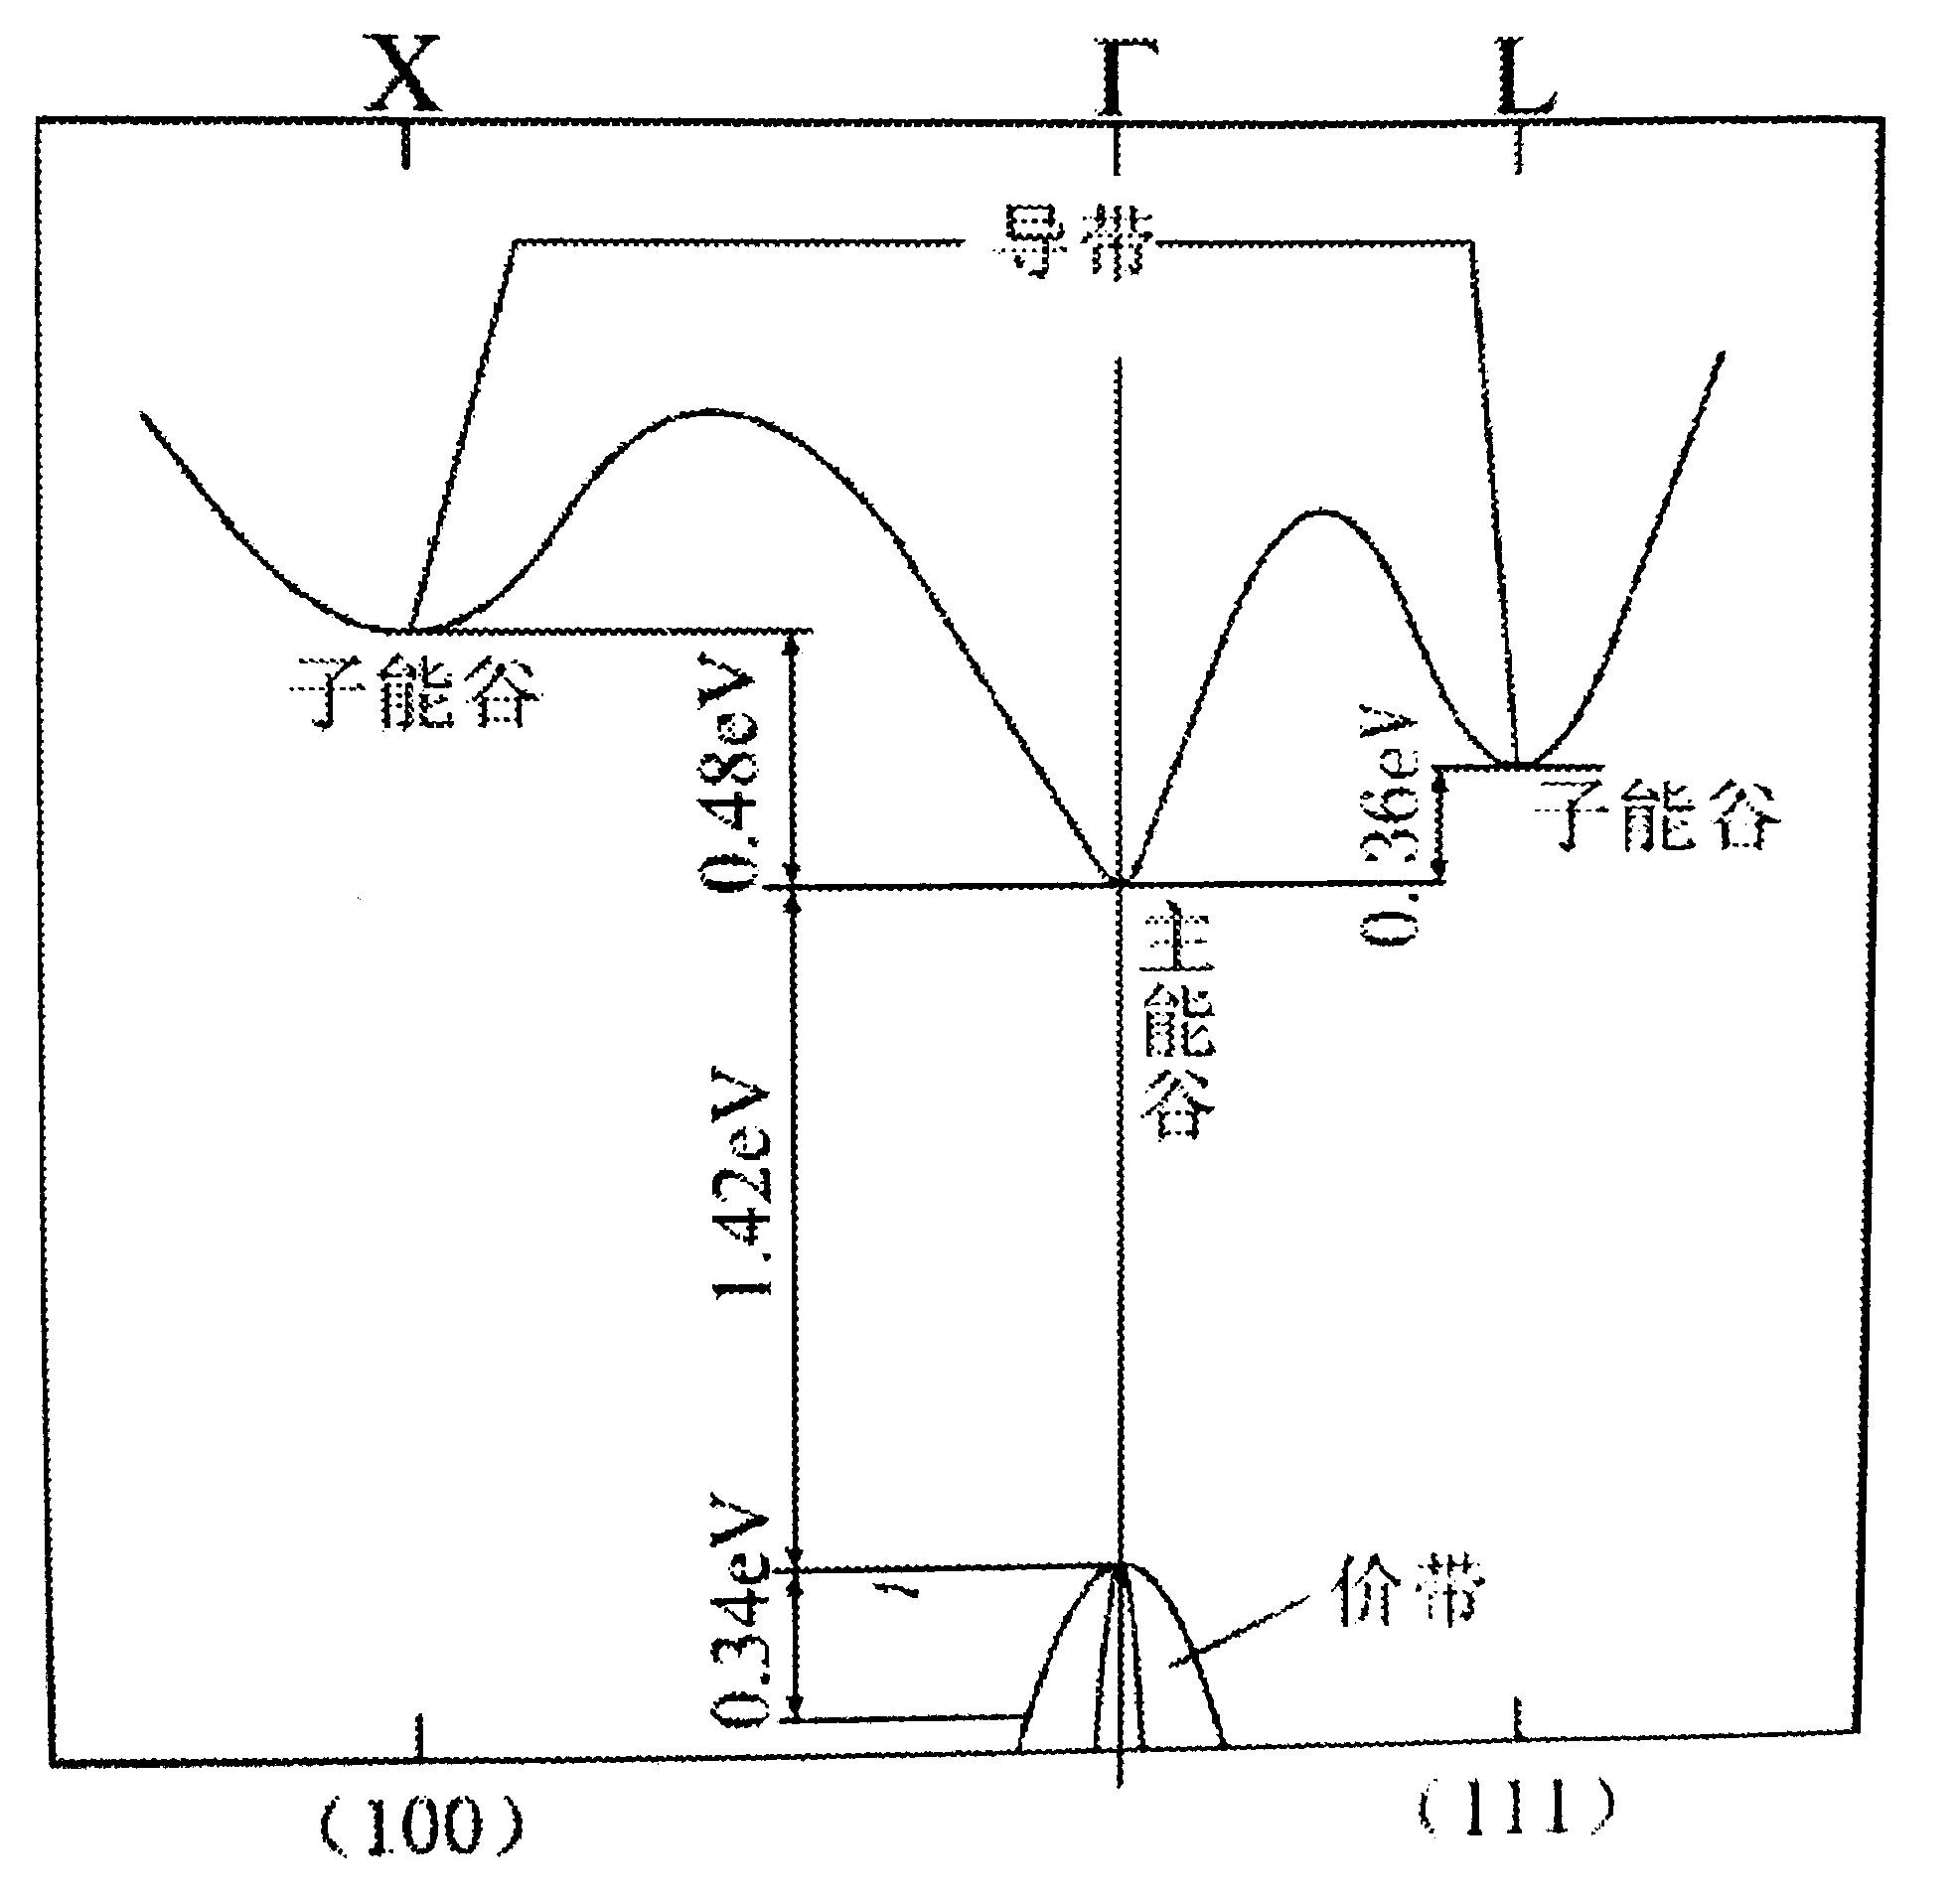
\includegraphics[width=4cm]{./fig/scan/EnergyBandStructureofGaAs.png}\caption{砷化镓的能带结构\label{fig:砷化镓的能带结构}}
		\end{wrapfigure}
		\FloatBarrier
		\par 一般采用微波固体振荡器或微波电子管产生微波;前者包括微波晶体管振荡器/体效应管振荡器等,而后者包括磁控管等,多用于需要较高微波功率的应用场景。本实验中用微波体效应管产生微波。
		\par 微波体效应管振荡器即耿氏二极管振荡器主要利用有双能谷结构的半导体材料的负阻特性形成的电流震荡输出微波。这类材料包括砷化镓/磷化铟/碲化镉/硒化锌/砷化铟等。以下以砷化镓为例。
		\par 300K下,砷化镓的能带结构如\cref{fig:砷化镓的能带结构}。图中可见其导带中的主能谷附近还有子能谷;能量最低的子能谷能量比主能谷高出约0.36eV,故其中电子迁移率(电子散射频率)小于主能谷。常温下电子能量不足以进入子能谷;加外电场到$E>E_{\rm th}$时,部分电子被激发到子能谷中,于是平均电子迁移率将下降,材料电阻下降,表现负阻特性;待电场增大到全部电子都被及发到子能谷中时,效应结束。
		\par 设晶体管阴极附近有一因接触电阻和杂质不均匀分布产生的电阻率较大的区域,则在晶体管两端加逐渐增大的电压时,此区域分压较大,电场较强,首先超过阈值电场,表现负阻特性,电子迁移率较低;于是其阴极一侧电子堆积,阳极一侧电子抽空,内部电场进一步增大,形成高场畴。由于总电压由外电路给定,此畴一旦形成,即将抑制其他区域的电场增大,故只会产生一个高场畴。
		\par 高场畴中电子仍将在电场作用下向阳极运动,故整个高场畴将向阳极渡越;同时,畴内电场增大使得内部电子迁移率重新增大,逐渐又与外部的迁移率相等;于是畴内电场不再增大,场畴成为成熟畴;成熟畴将稳定地渡越到阳极,在阳极被吸收后在电路激起一个电流脉冲,同时晶体管内开始下一个畴的形成。\supct{bib:textbook}
		\par 在上述过程中,砷化镓表现如\cref{subfig:体效应管的电流-电压特性}的电流-电压特性。当电压$V$小于阈值电压$V_{\rm th}$时,高场畴尚未形成,通过晶体管的电流与其两端的电压成正比。到达A点时,两端电压接近阈值电压后,高场畴开始形成,整体电阻随总电压增长而下降;达到C点后形成成熟畴,电流随着电压增长又略有上升。到达D点后再降低电压,则在B点后畴内电场仍高于阈值,高场畴仍可维持,直到总电压小于$V_{\rm s}$(维持电压)时,高场畴不能维持,电流跃变到与上升阶段相同的位置F。
		\begin{figure}[htbp]
			\subfloat[高场畴的形成(图a-b),渡越(图b-c)与消失(图d)]{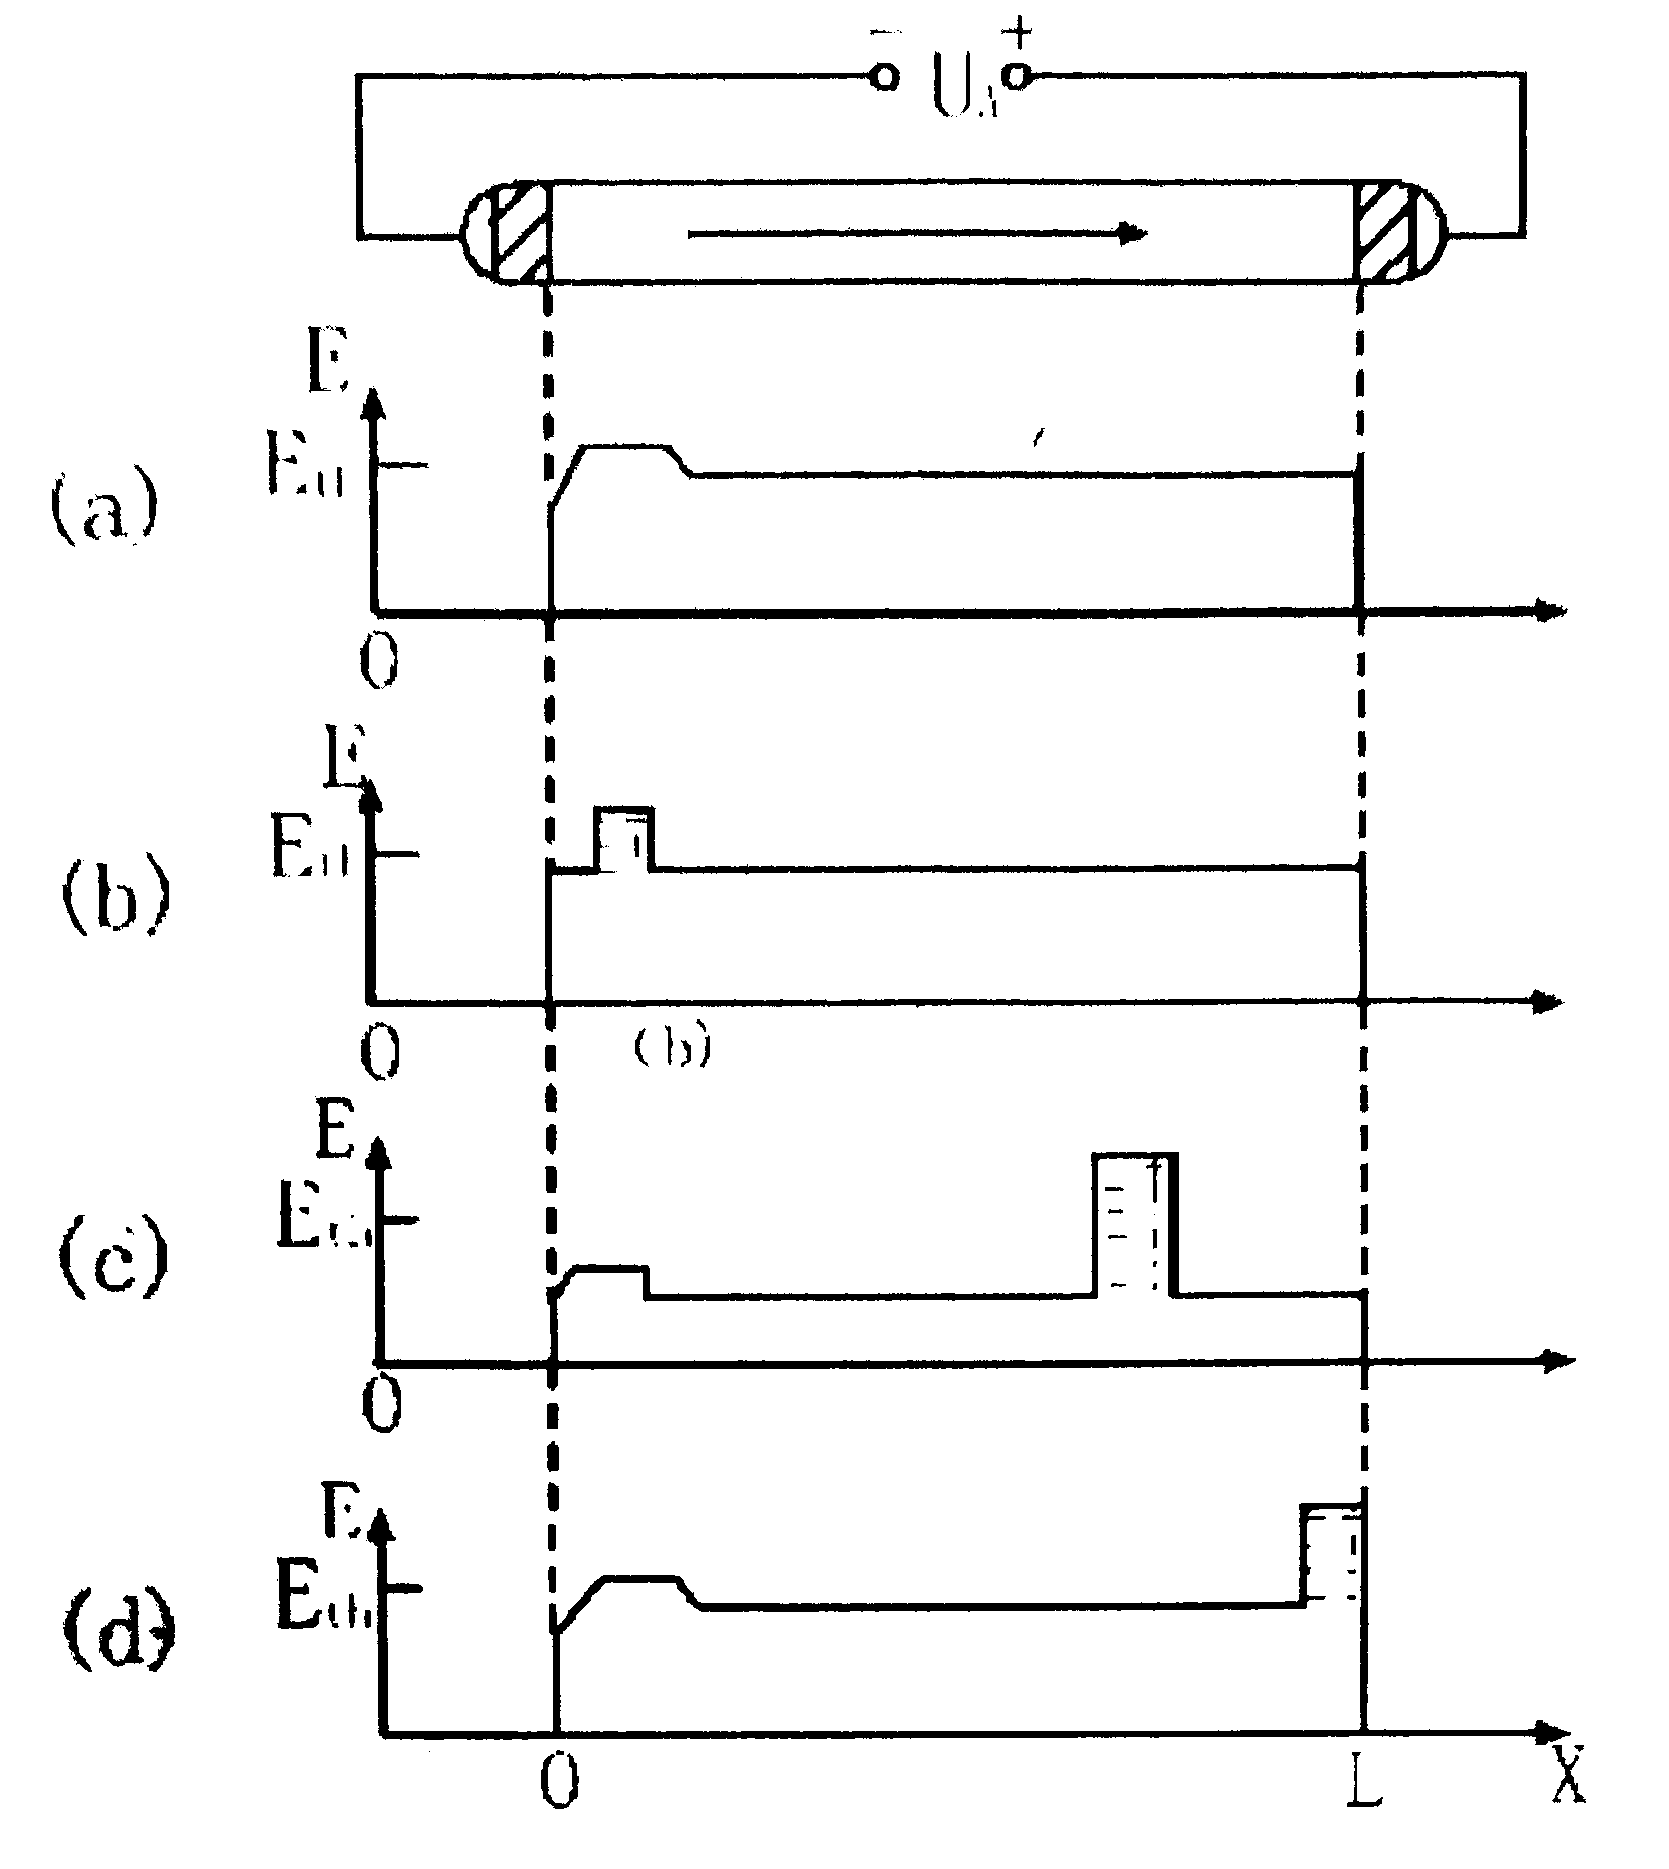
\includegraphics[height=5cm]{fig/scan/LifespanofaHighFieldDomain.png}\label{subfig:高场畴的形成,渡越与消失}}\quad
			\subfloat[体效应管的电流-电压特性]{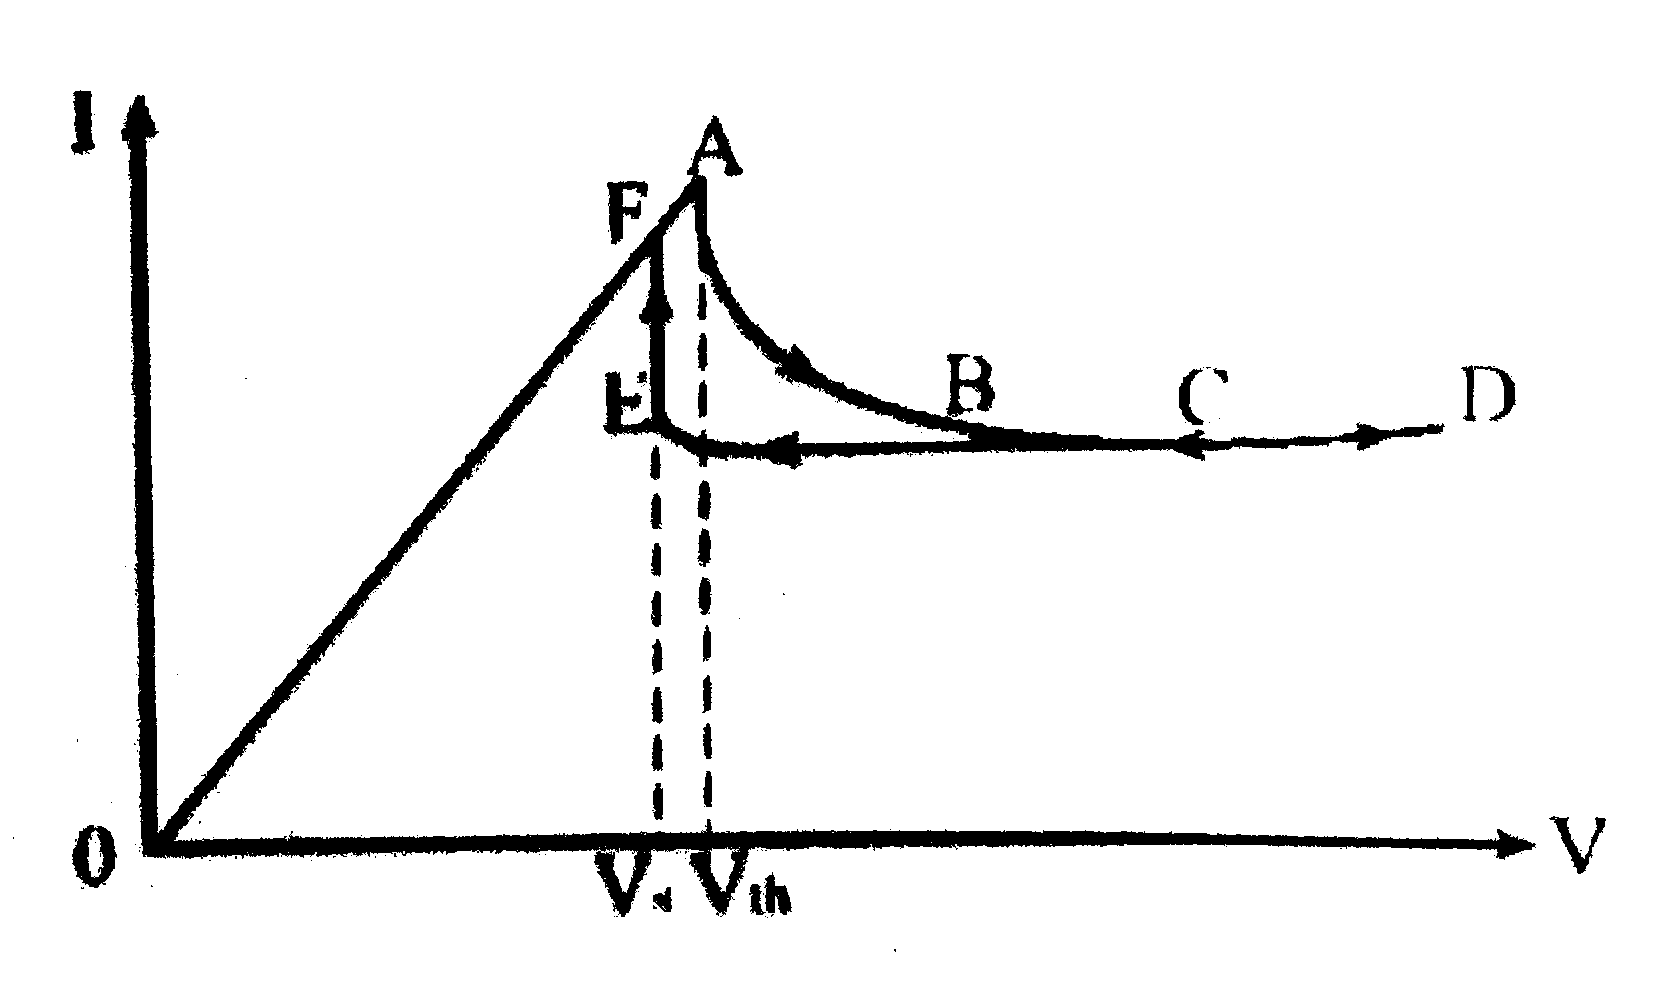
\includegraphics[height=5cm,width=5cm]{fig/scan/I-VFeatureofaBodyEffectTube.png}\label{subfig:体效应管的电流-电压特性}}\quad
			\subfloat[体效应二极管的工作原理]{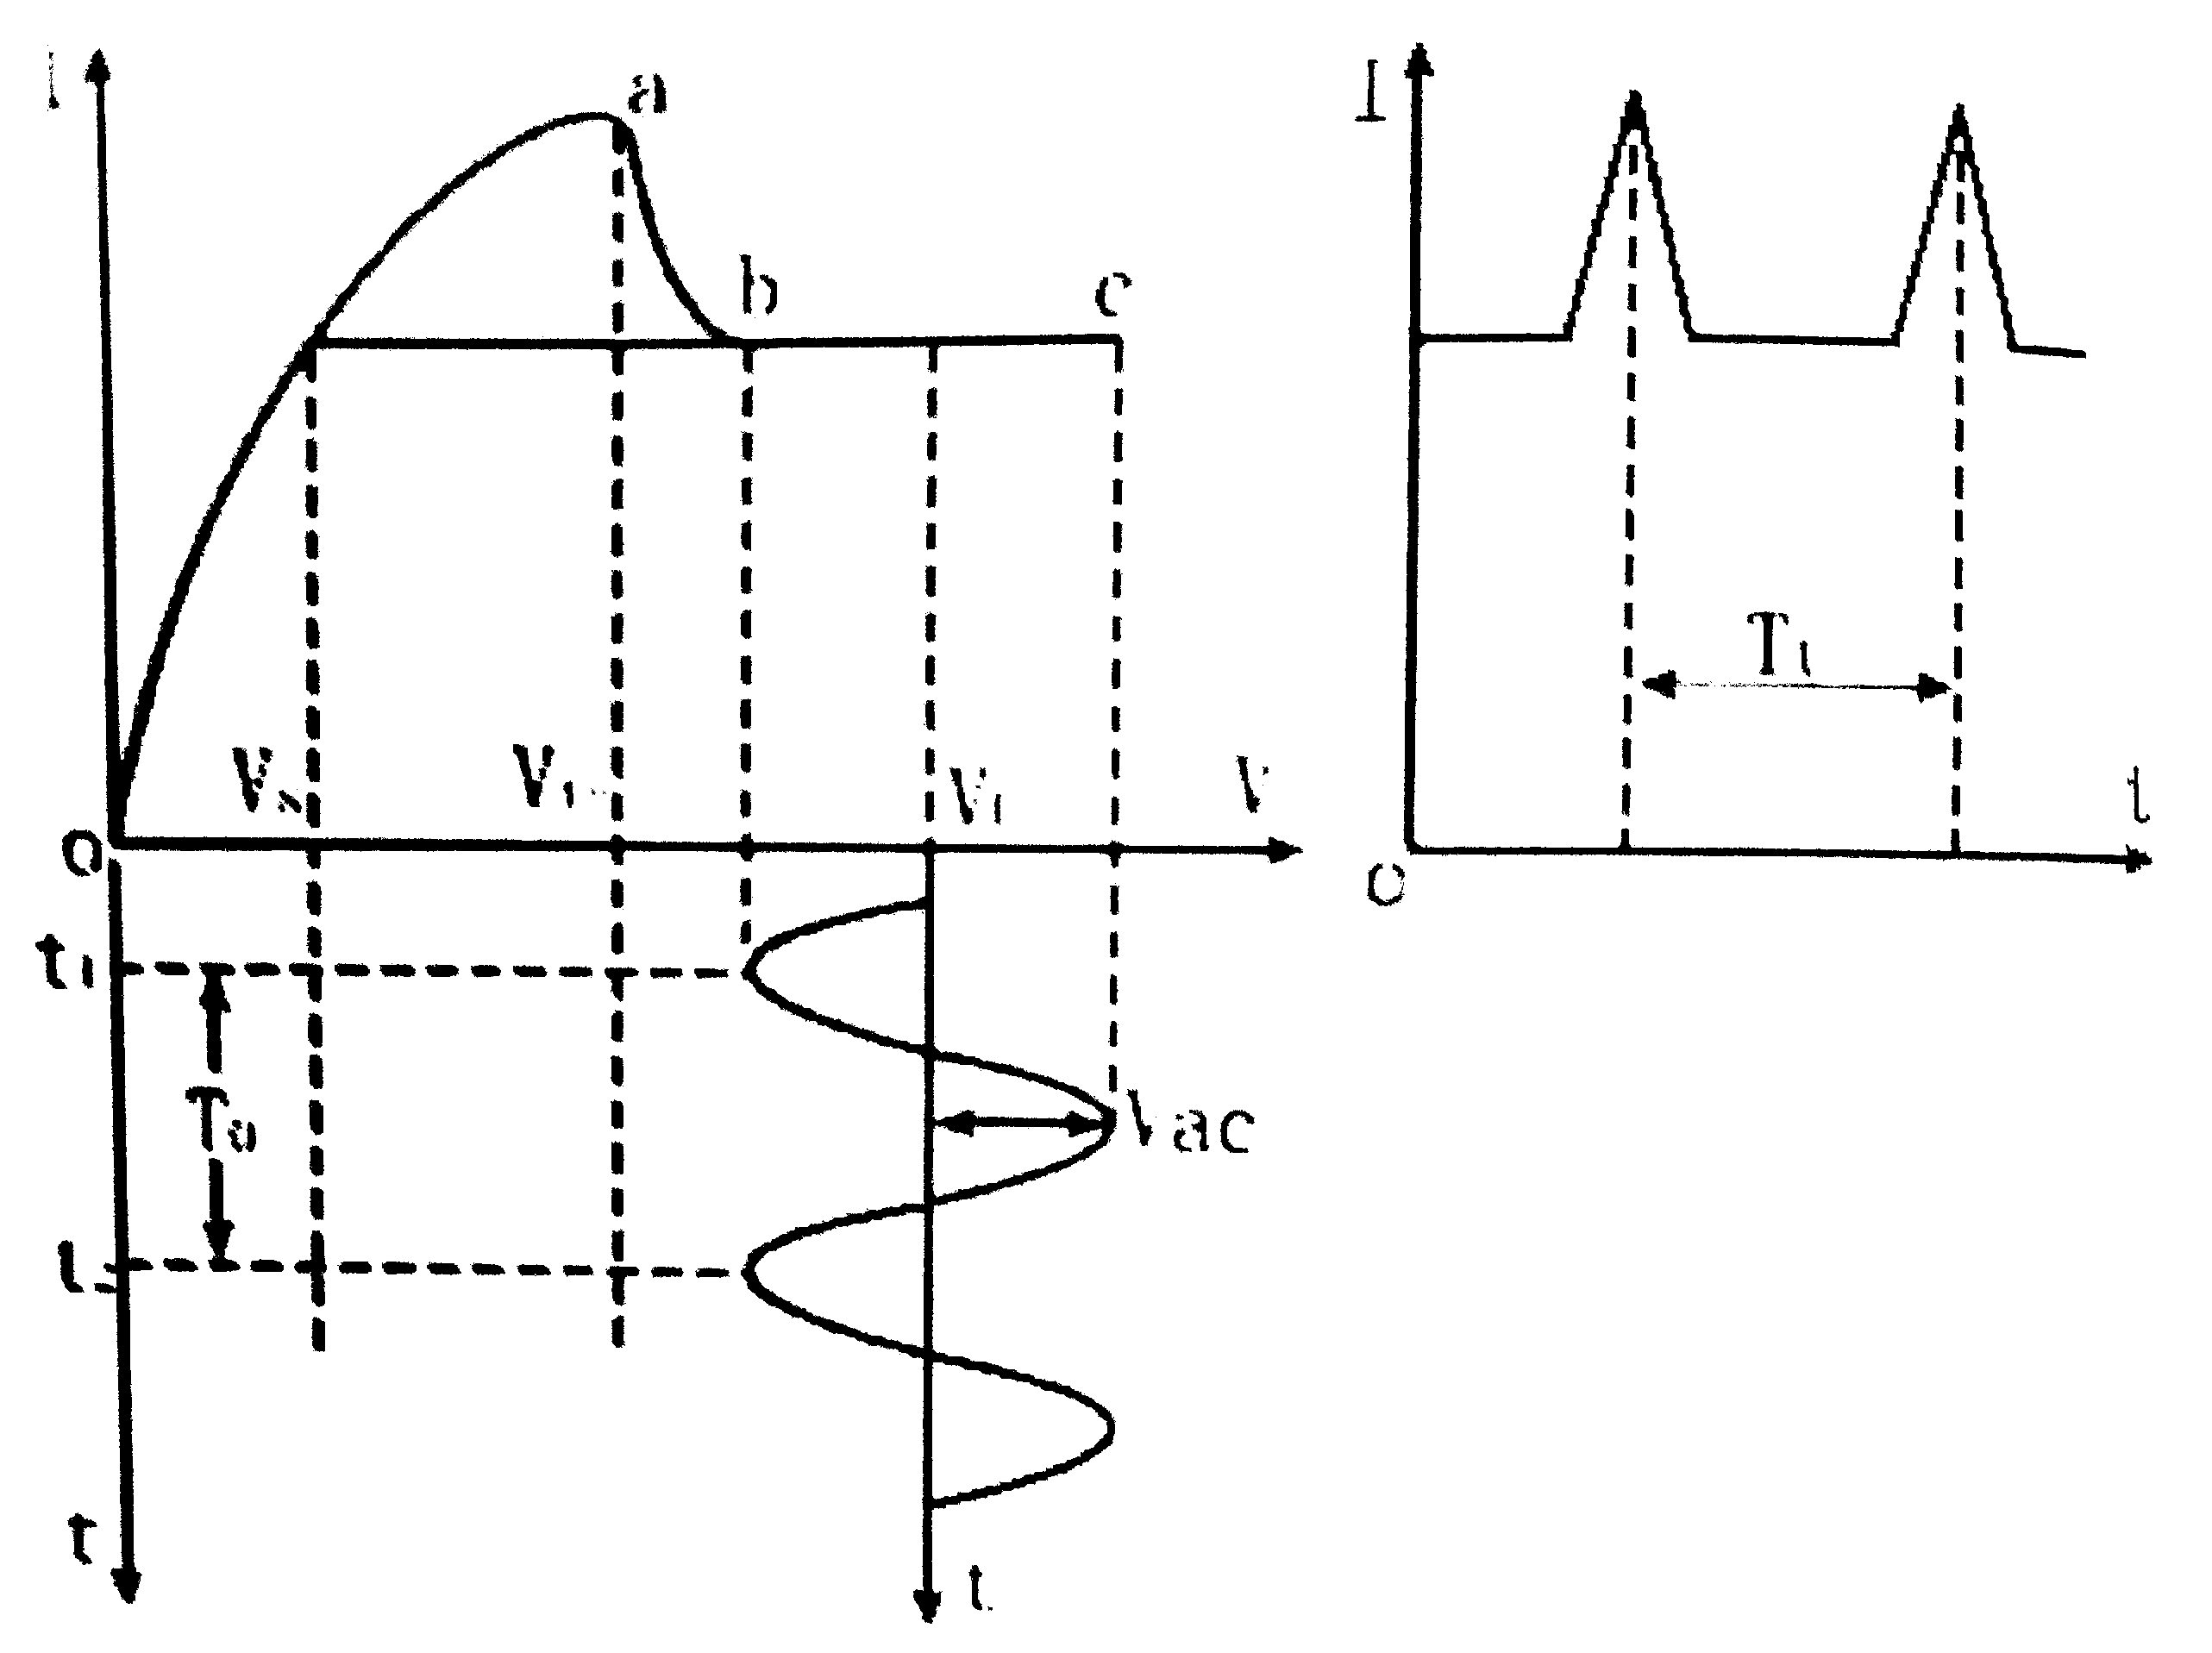
\includegraphics[height=5cm]{fig/scan/PrinciplesofWorkingofaBodyEffectDiode.png}\label{subfig:体效应二极管的工作原理}}
			\caption{体效应二极管}\label{fig:体效应二极管的工作原理}
		\end{figure}
		\par 通过外电路向体效应管提供振荡电压$V=V_{\rm b}+V_{\rm ac}\cos{\omega_0 t}$,并令$V_{\rm b}-V_{\rm ac}>V_{\rm th}$(\cref{subfig:体效应二极管的工作原理})。电压零开始上升的过程激发了最初的一次振荡:在外电压最小时高场畴即可开始形成并向阳极渡越,到下一个最小值时被阳极吸收,形成一个电流脉冲,同时下一个高场畴开始成核。晶体管与外电路相互作用,就形成了频率为$\omega_0$的一组电流脉冲。\supct{bib:textbook}晶体管与外电路的阻抗的实部与虚部则分别决定了电路的频率与功率。
	% subsubsection 微波的产生 (end)
	\subsubsection{微波的传播} % (fold)
		\label{ssub:微波的传播}
		\FloatBarrier
		\begin{wrapfigure}[]{r}[0pt]{4cm}
			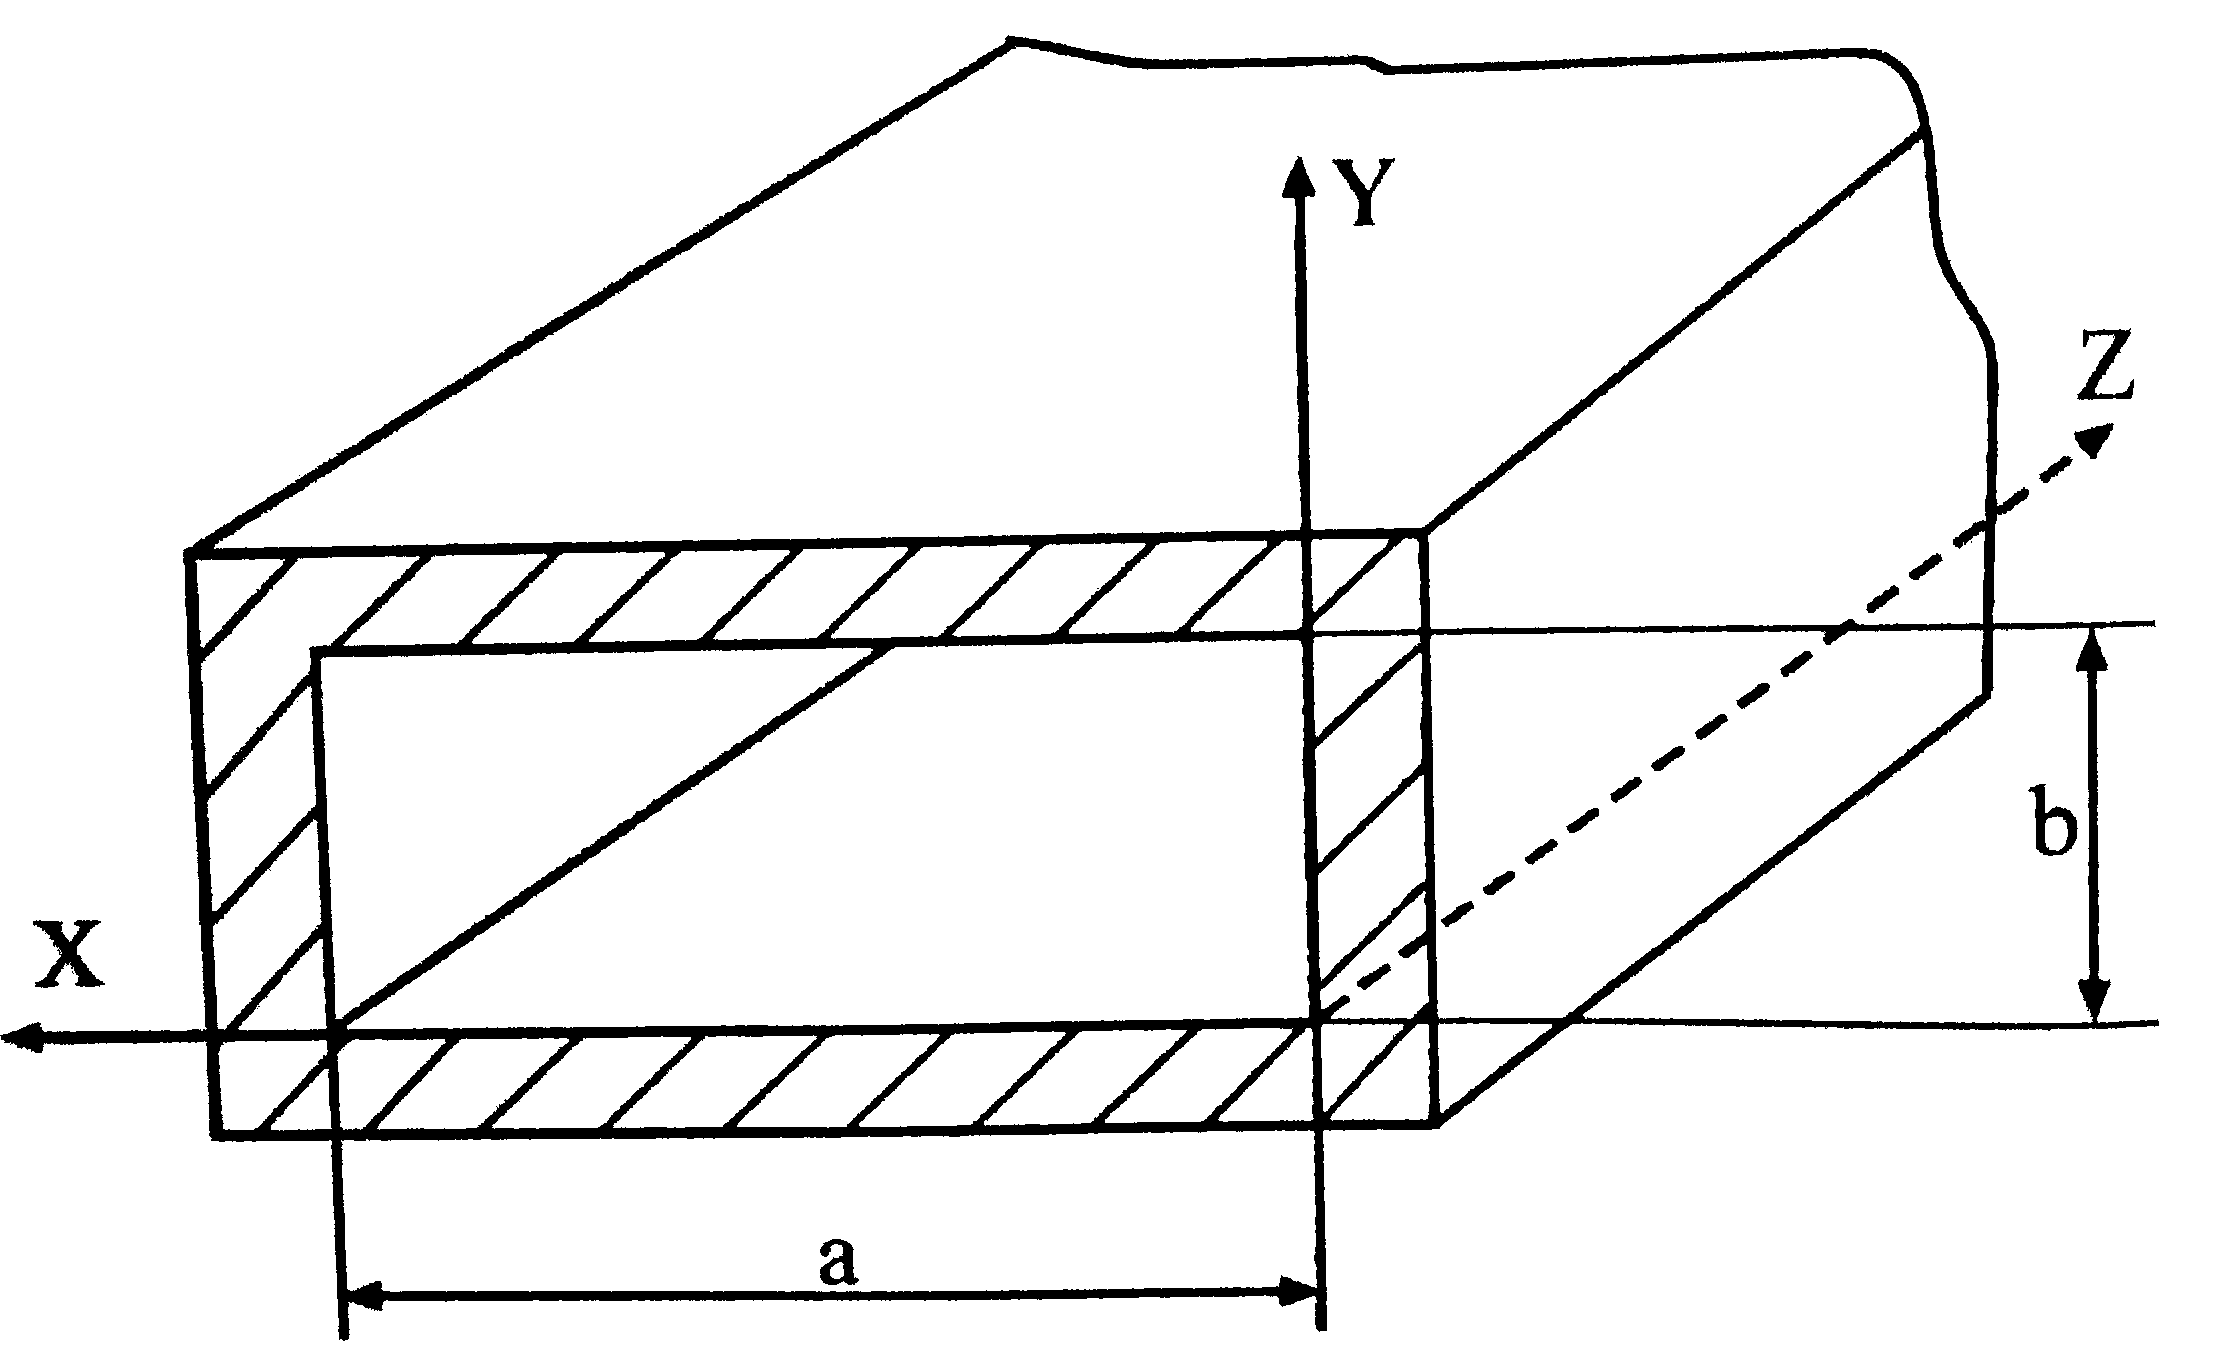
\includegraphics[width=3cm]{fig/scan/Rectangularwaveguide.png}
			\caption{矩形波导管}\label{fig:矩形波导管}
		\end{wrapfigure}
		\FloatBarrier
		\par 波导管是一段中空金属管。波导管中传播的电磁波一定由纵向分量,但没有横向电场分量或横向磁场分量,分别称为横磁波(TM)/横电波(TE)。同时有电磁场横向分量的微波(TEM)只能在多层金属组成的电缆中传输。标准的矩形波导管只传输TE波,没有纵向电场。
		\par 设有均匀无限长无损耗$a\times b$矩形波导管,其中介质均匀,介电常数为$\varepsilon$,磁导率为$\mu$,一端输入角频率为$\omega$的代电磁波,沿$z$轴方向传播(方向如\cref{fig:矩形波导管}所示)。其中TE$_{10}$波解为
		\begin{equation}
			\begin{cases}
				E_y=E_0\sin{\dfrac{\pi x}{a}}{\rm e}^{{\rm i}(\omega t-\beta z)},\quad E_x=E_y=0;\\
				H_x=-\dfrac{\beta}{\omega\mu}E_0\sin{\dfrac{\pi x}{a}}{\rm e}^{{\rm i}(\omega t-\beta z)},\quad H_y=0,\\
				H_z={\rm i}\dfrac{\pi}{\omega\mu a}E_0\cos{\dfrac{\pi x}{a}}{\rm e}^{{\rm i}(\omega t-\beta z)}.
			\end{cases}\label{eq:emwave}
		\end{equation}
		\FloatBarrier
		\begin{wrapfigure}[]{r}[0pt]{6cm }
			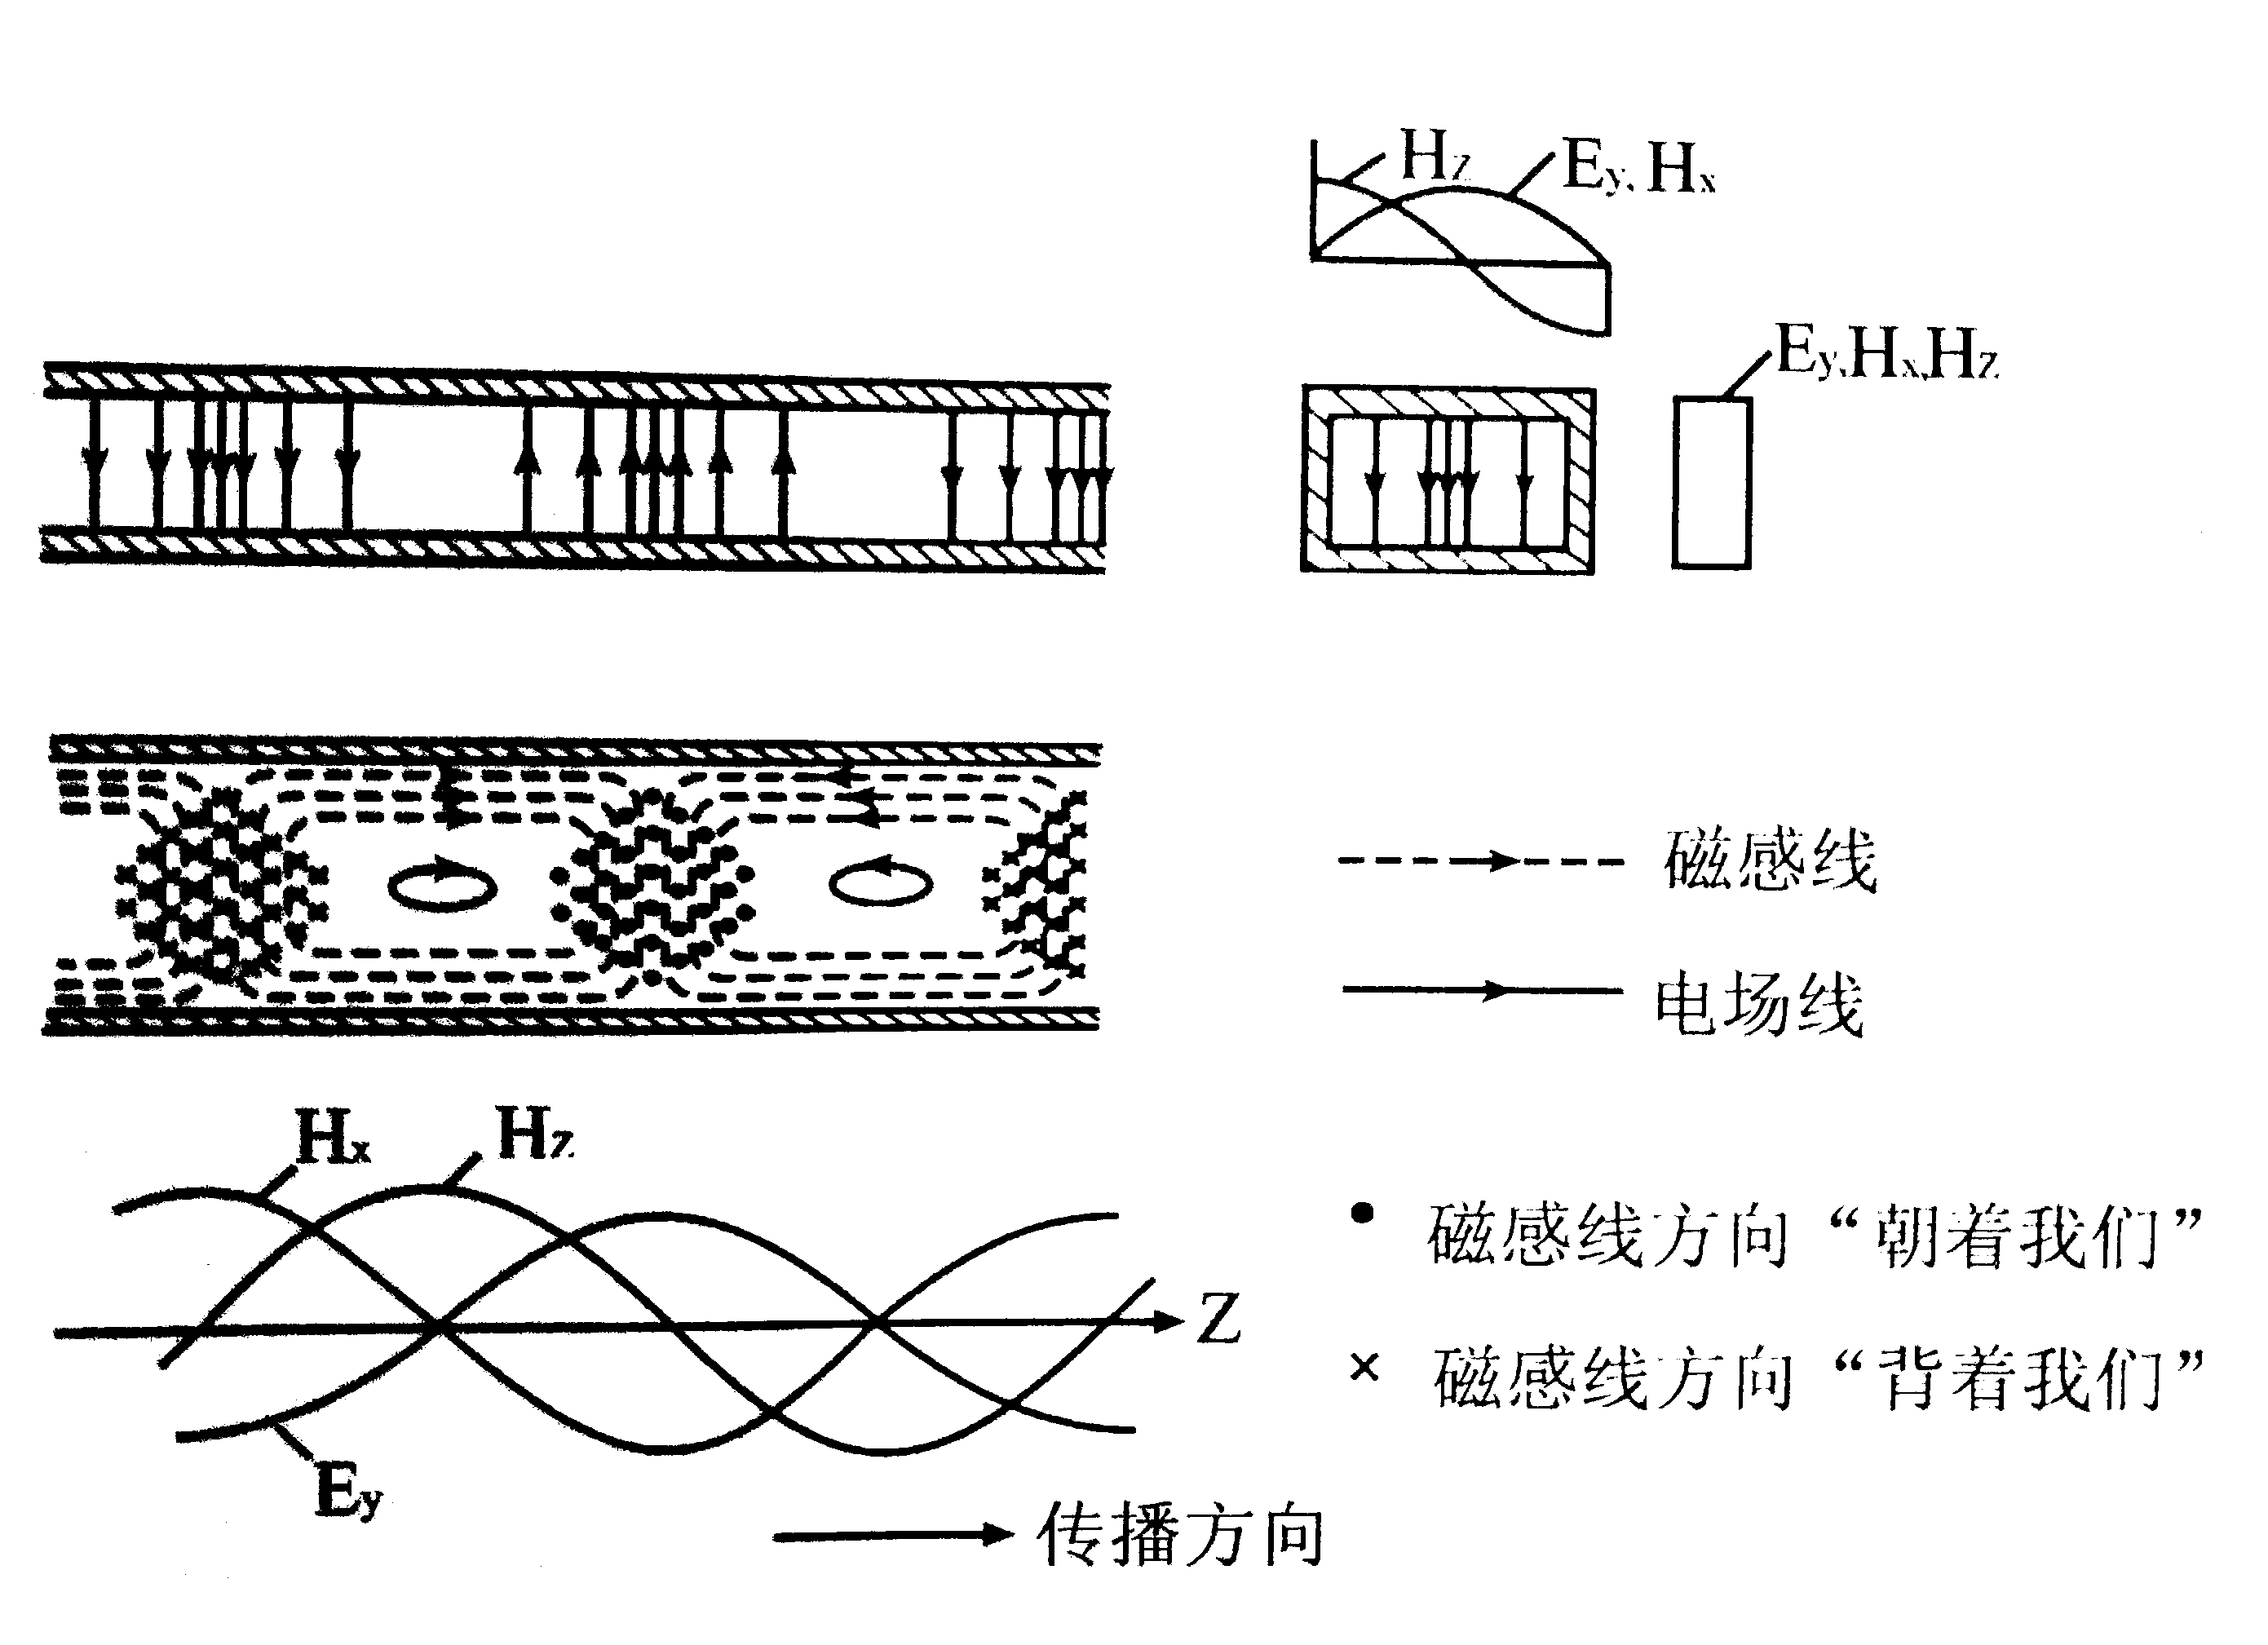
\includegraphics[width=5cm]{fig/scan/StructureoftheEMFieldofTE10Wave.png}
			\caption{波导管中TE$_{10}$波的电磁场结构}\label{fig:波导管中TE10波的电磁场结构}
		\end{wrapfigure}
		\FloatBarrier
		其中,
		\begin{equation}
		\begin{aligned}
			&\beta =\dfrac{2\pi}{\lambda_{\rm g}}\text{是相位常数}\text{,波导波长}\lambda_{\rm g}=\dfrac{\lambda}{\sqrt{1-\left(\lambda /\lambda_0\right)^2}},\\
			&\lambda_0 = 2a,\lambda\text{是微波在真空中的波长。}
		\end{aligned}\label{eq:beta}
		\end{equation}
		
		\par 由\cref{eq:emwave}可以看出此波导管中的电磁波分布具有以下特征:
		\begin{enumerate}
			\item $\lambda_{\rm g} >\lambda$;
			\item 只有$\lambda <\lambda_0=2a$的电磁波可以在此波导管中传输;
			\item $\boldsymbol{E}\parallelsym\hat{\boldsymbol{e}}_{y},\boldsymbol{H}\perp\hat{\boldsymbol{e}}_{y}$;
			\item 电场在$x$方向是驻立半波;
			\item $E_y$与$H_x$分布情况相同,相位相差为$\pi$。磁场的这种结构是行波的特点(\cref{fig:波导管中TE10波的电磁场结构})。
		\end{enumerate}
	% subsubsection 微波的传播 (end)
	\subsubsection{微波测量} % (fold)
		\label{ssub:微波测量}
		\begin{figure}[htbp]
			\subfloat[谐振式频率计]{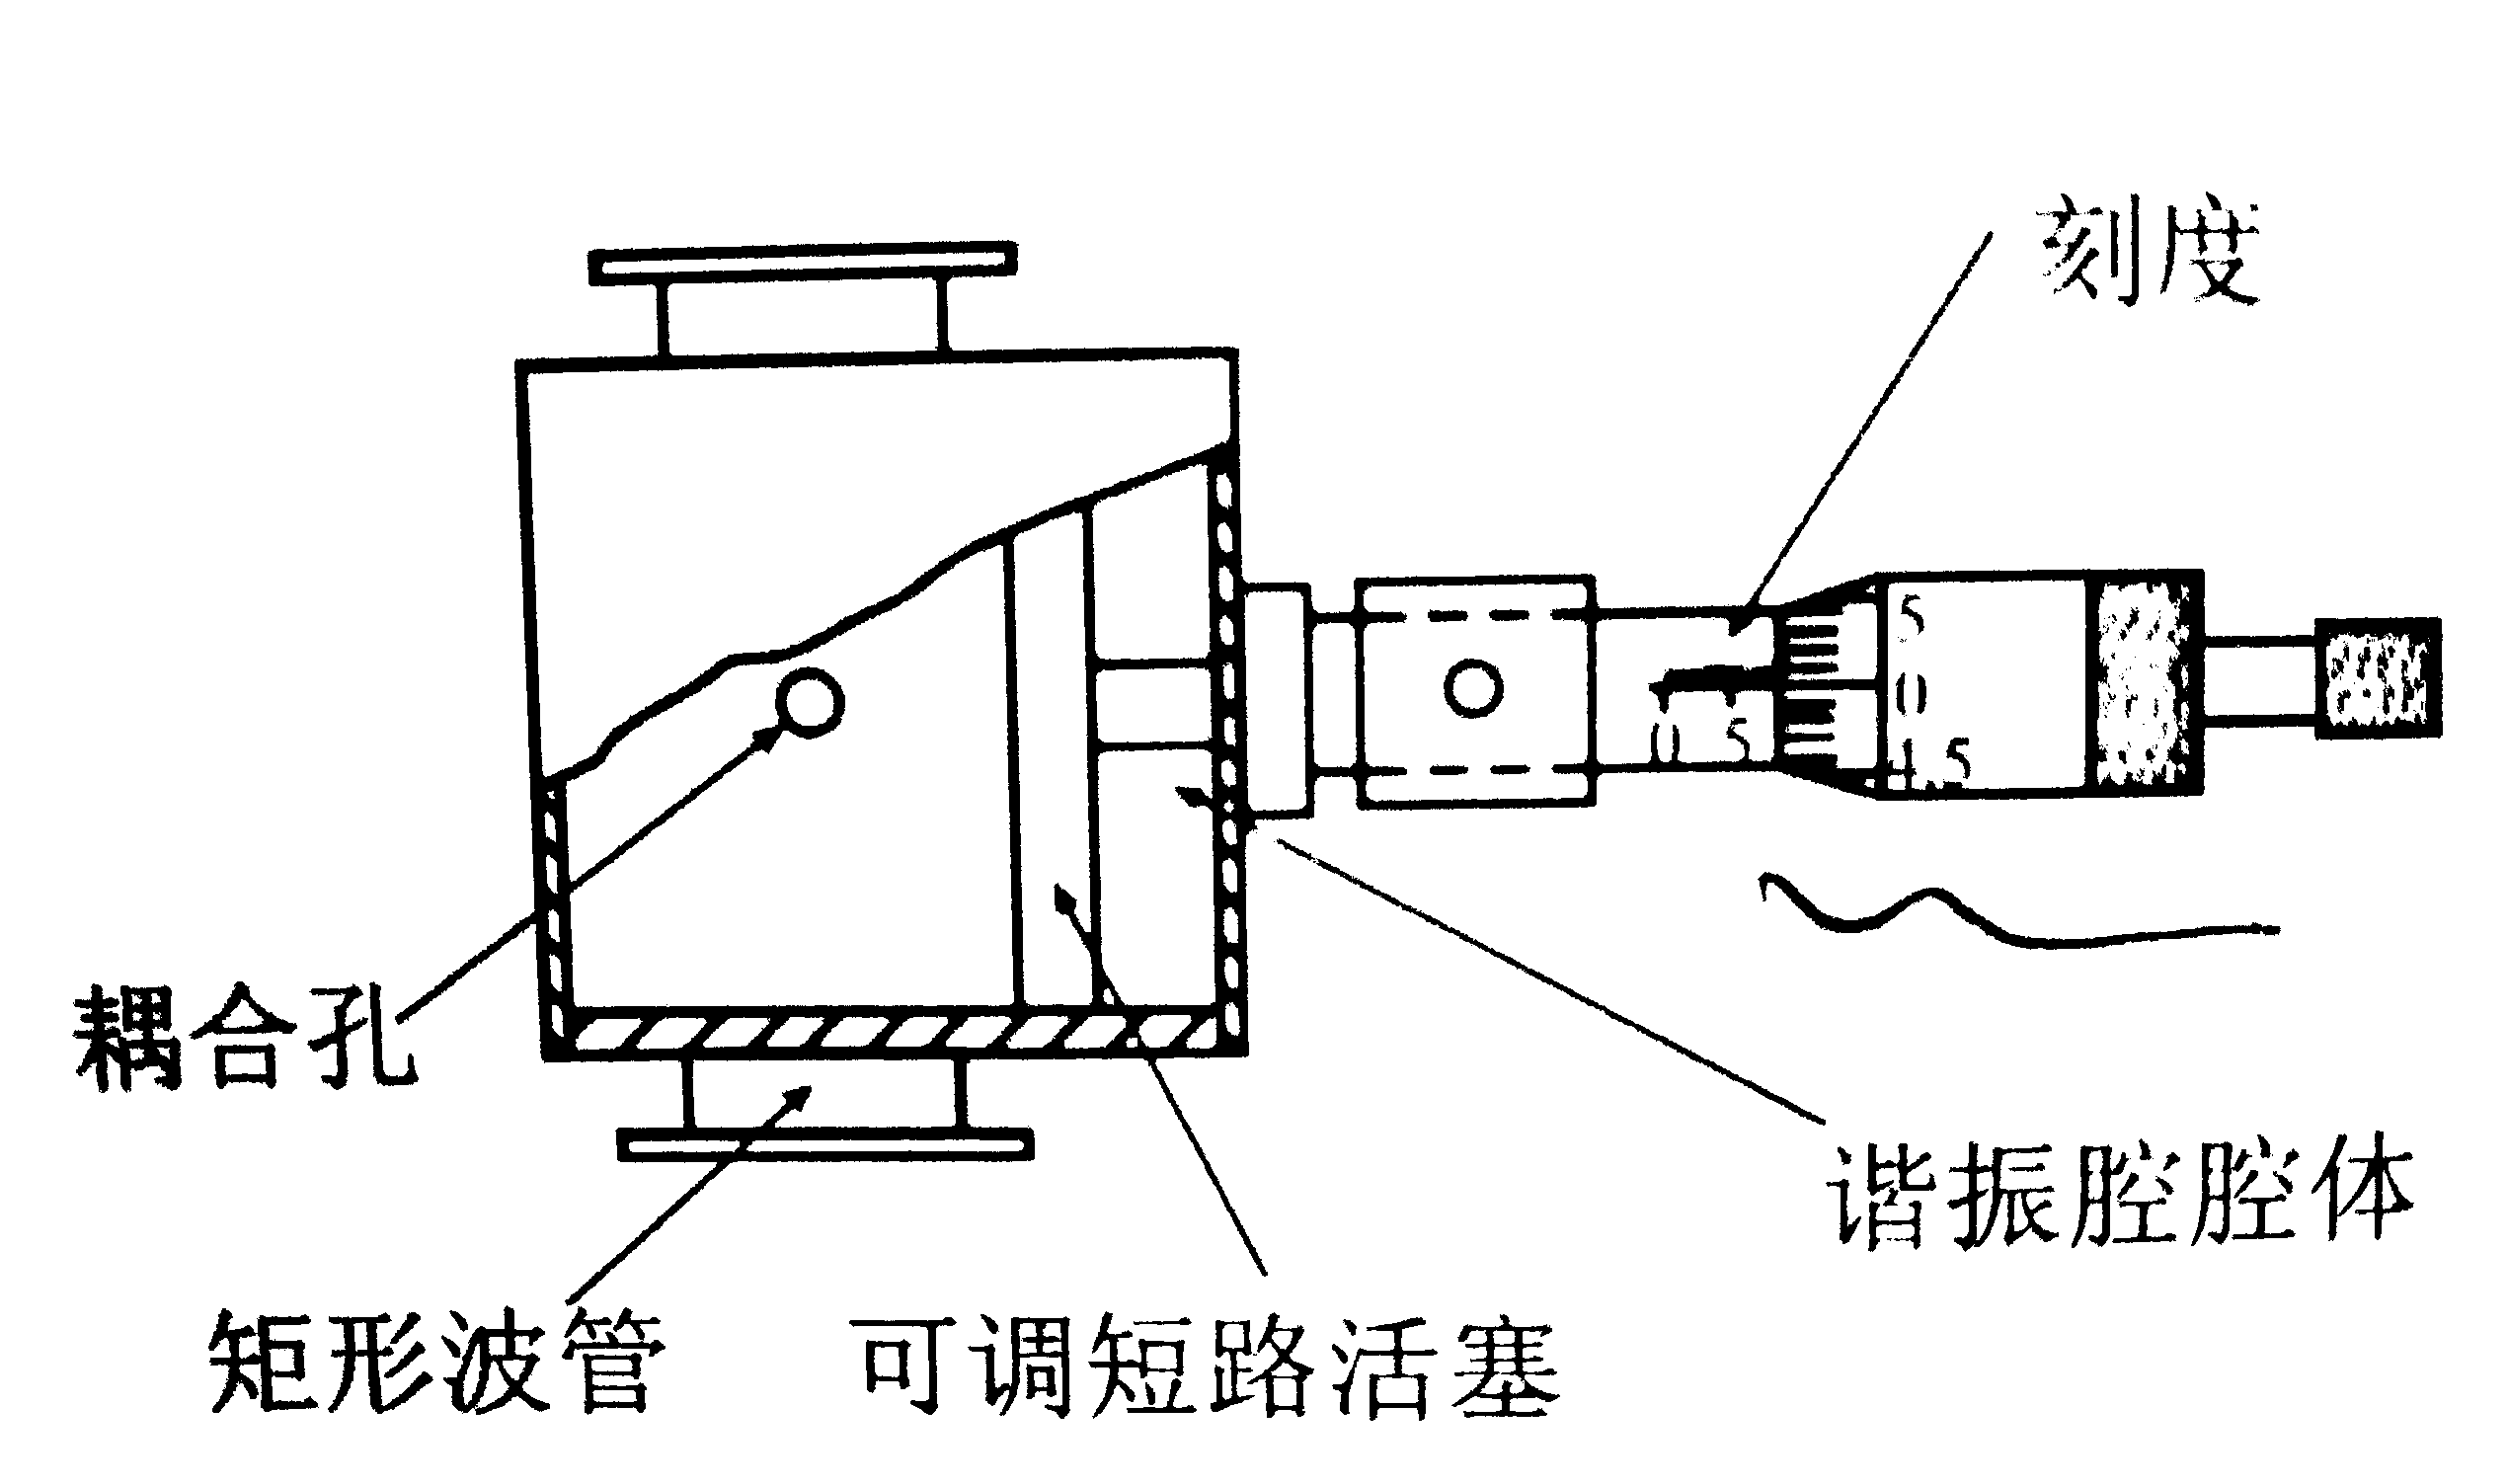
\includegraphics[height=3cm,width=4cm]{fig/scan/StructureofaResonaceSpectrometer.png}\label{subfig:谐振式频率计}}\hspace{.5cm}
			\subfloat[晶体检波器]{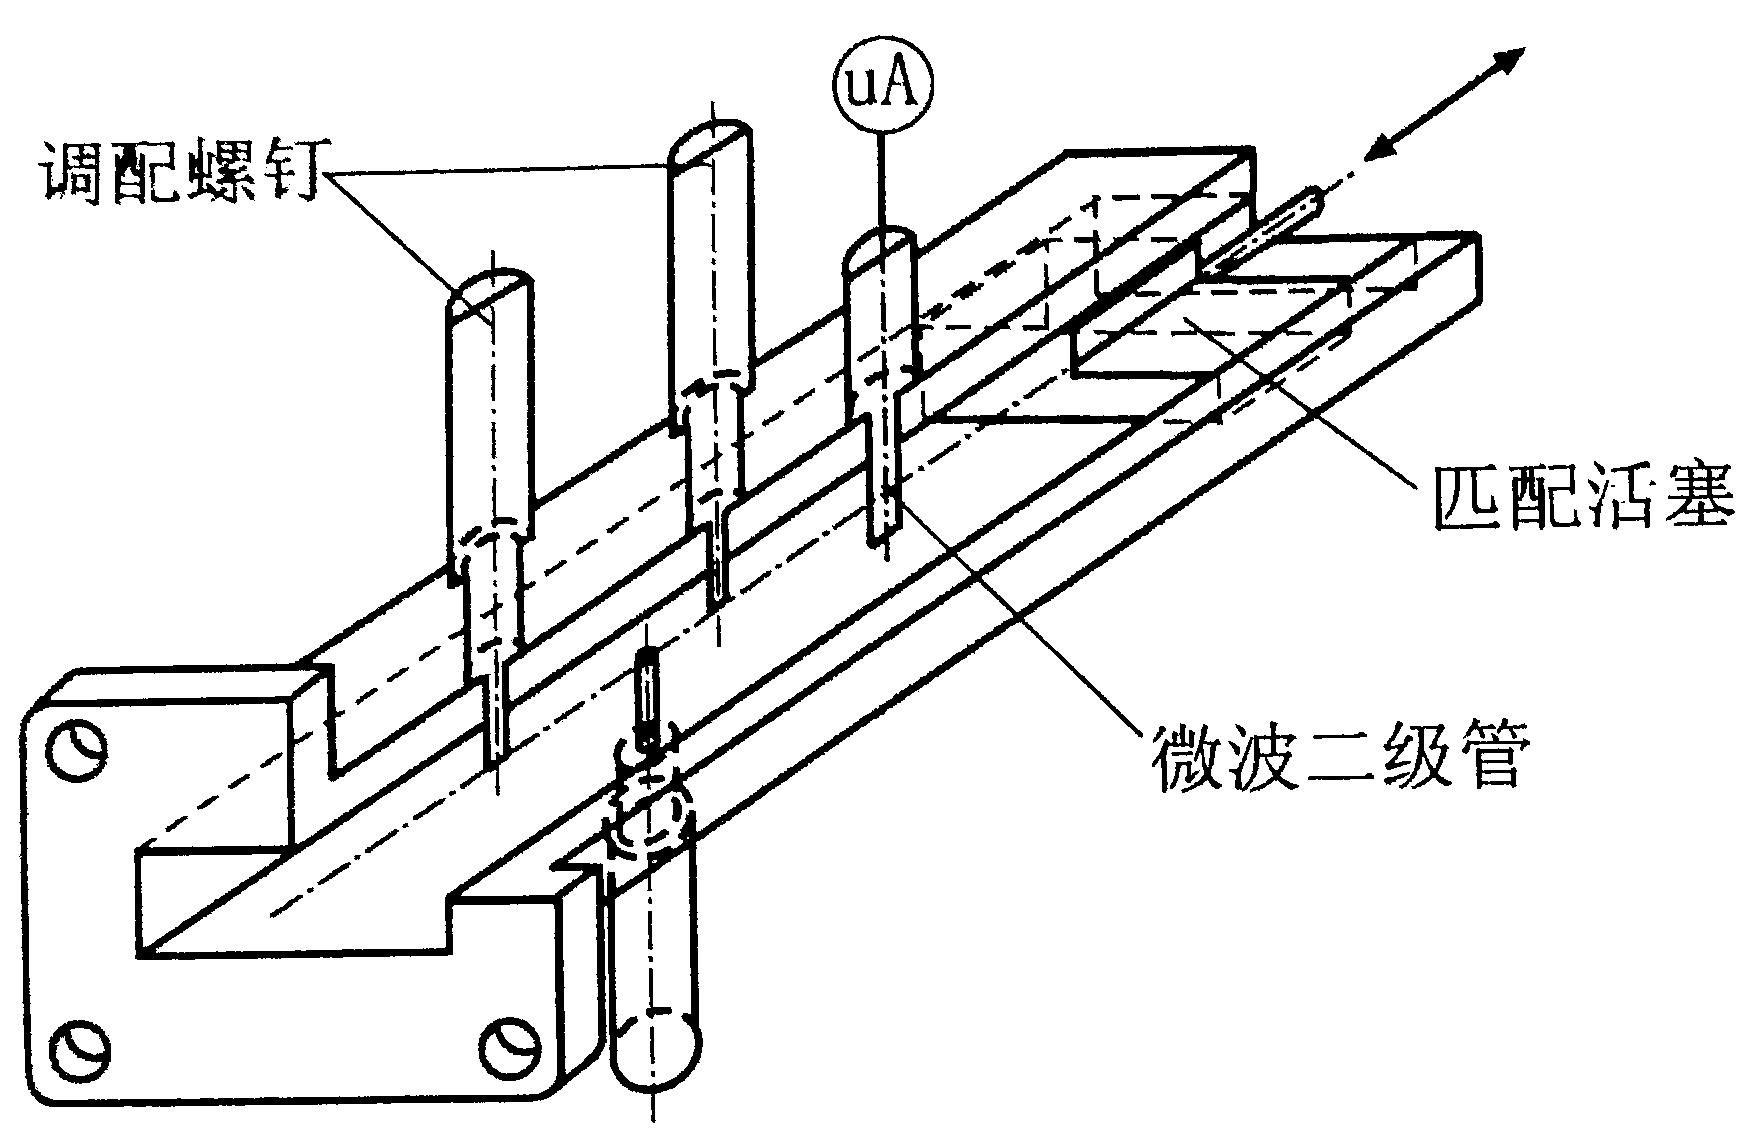
\includegraphics[height=3cm,width=4cm]{fig/scan/CrystalWaveDetector.png}\label{subfig:晶体检波器}}\hspace{.5cm}
			\subfloat[微波检波二极管的$I_V$曲线]{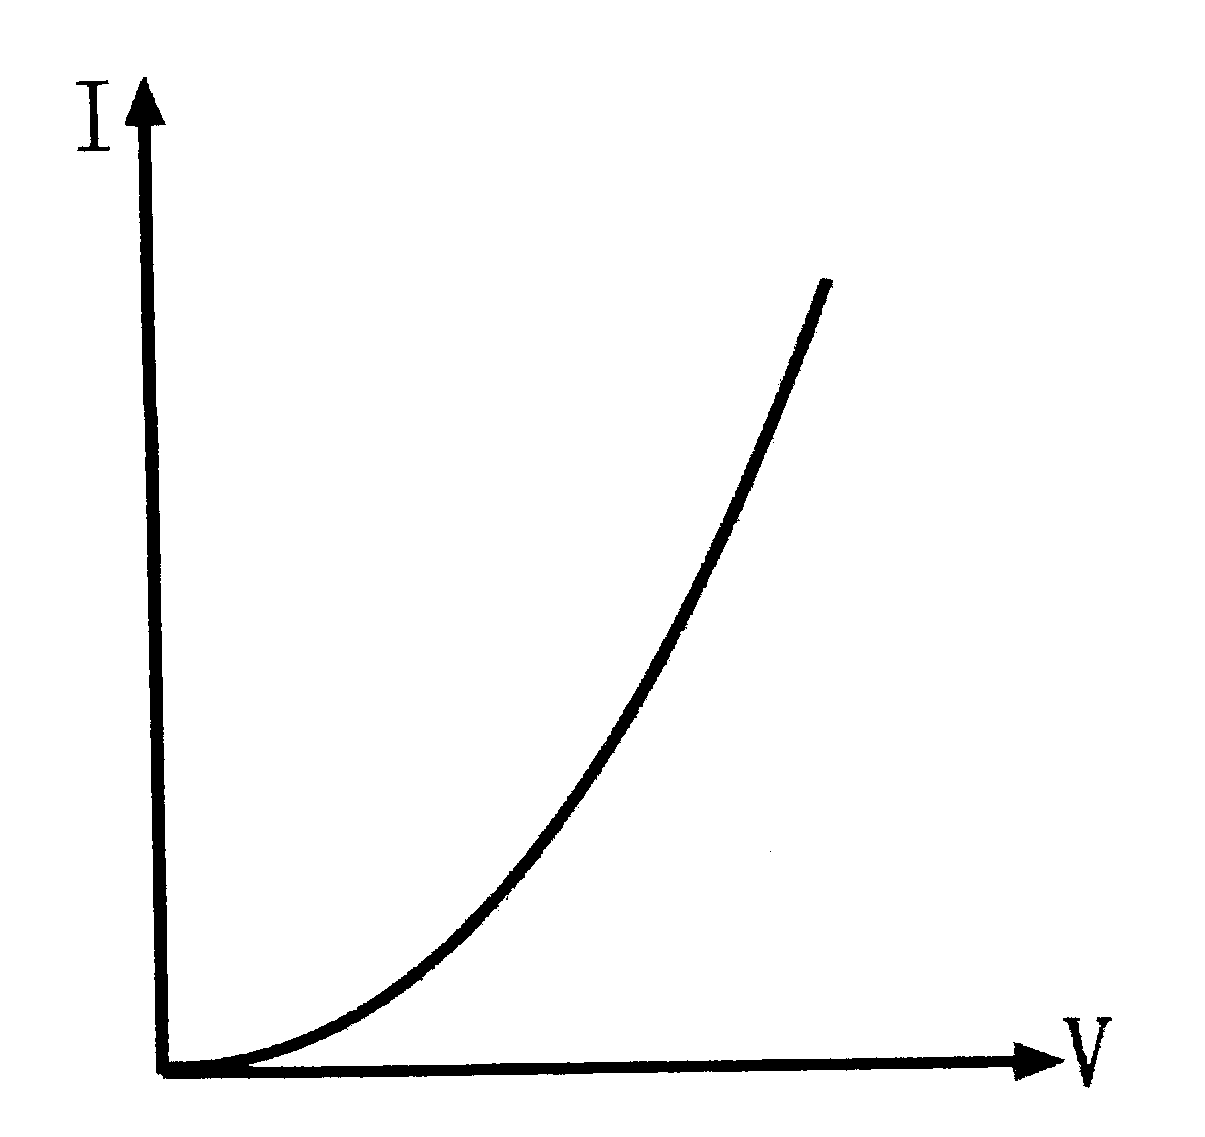
\includegraphics[height=3cm,width=3cm]{fig/scan/I-VCurveofaDetectorDiode.png}\label{subfig:微波检波二极管的IV曲线}}\hspace{.5cm}
			\subfloat[测量线]{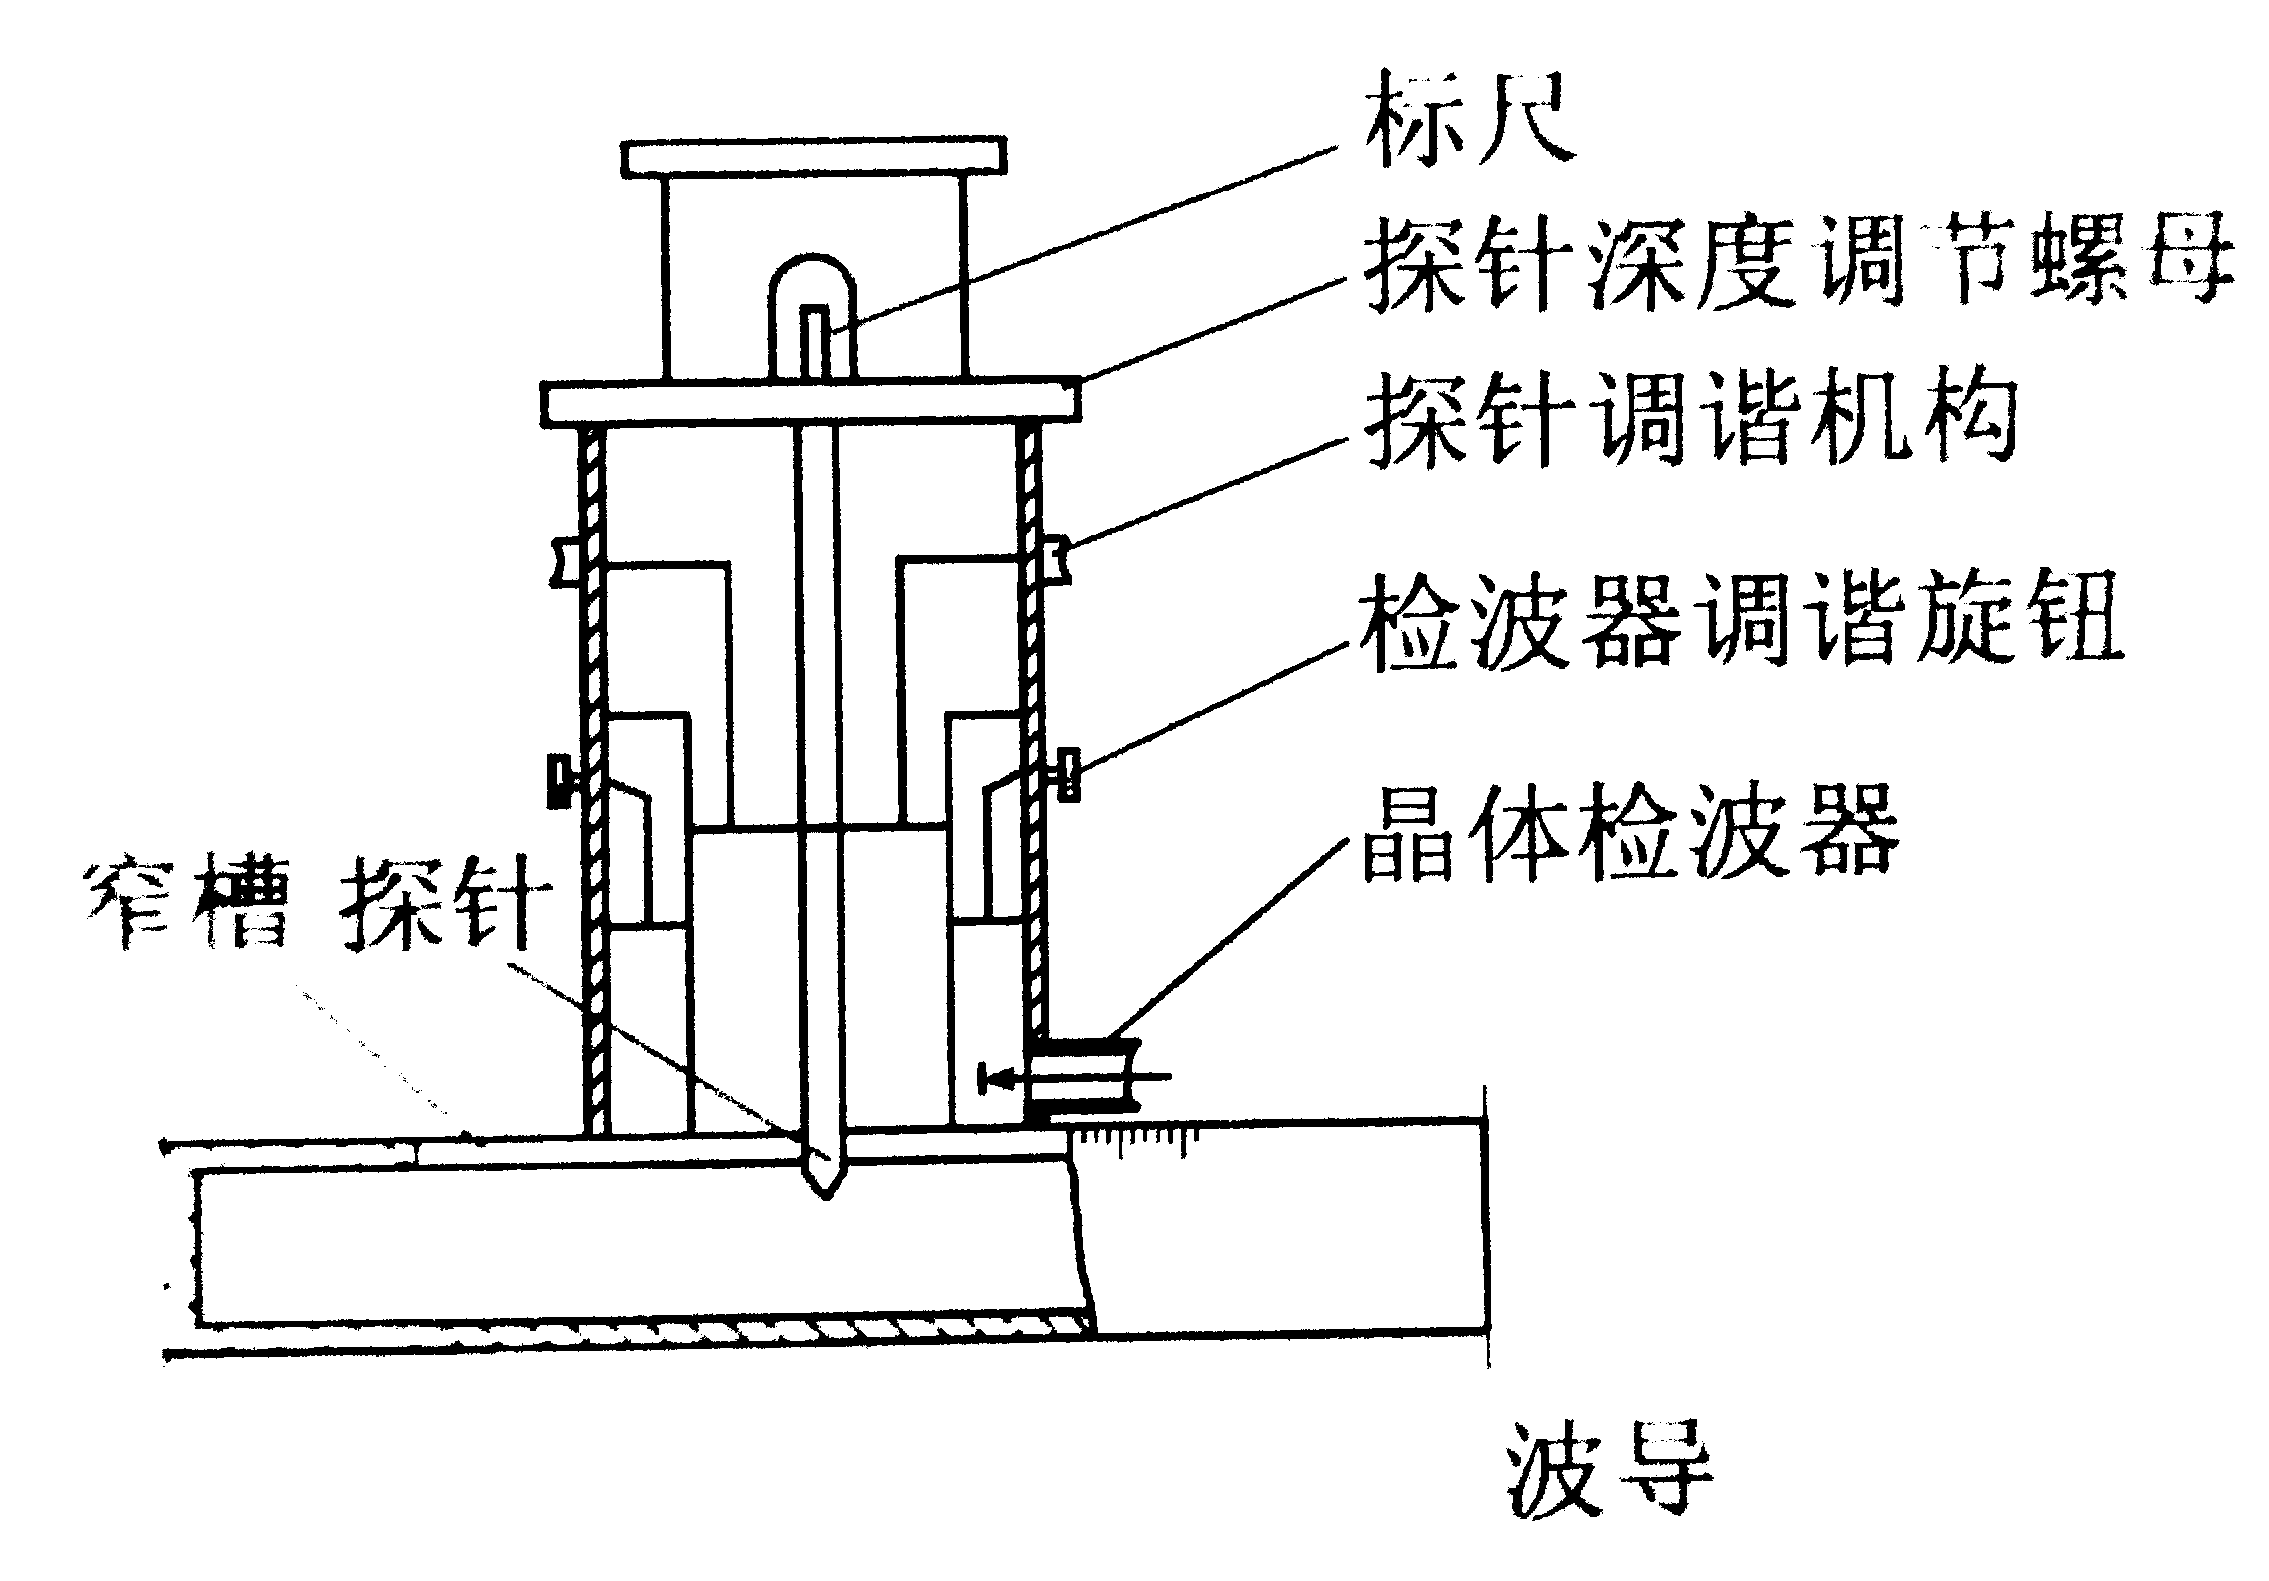
\includegraphics[height=3cm,width=4cm]{fig/scan/StructureofaMeasuringLine.png}\label{subfig:测量线}}
			\caption{微波测量}\label{fig:微波测量}
		\end{figure}
		\begin{enumerate}
			\item 频率测量(谐振式频率计)\\
				吸收式谐振频率计(\cref{subfig:谐振式频率计})是一个长度$L$可调的谐振腔,可以通过耦合孔与波导管相连,调节$L$至腔体对微波功率发生强烈的共振吸收,功率监测示数减小,即可通过频率校正表得到微波频率。
			\item 功率测量(晶体检波器)\\
				功率的绝对测量可以用热敏电阻等测量微波转化的热能,也可以用晶体检波器用于检测功率的相对值。晶体检波器(\cref{subfig:晶体检波器})中的微波二极管将微波信号转化为直流电信号,微波电信号很弱,处于非线性区;若微波检波信号电流在5$\sim 10\upmu$A,大致有$I\propto V^2$,即平方检波律(\cref{subfig:微波检波二极管的IV曲线}),由此可知$I=KP$,故可用$I$作为$P$的相对值。
			\item 驻波比测量(测量线)\\
				如\cref{subfig:测量线},在一段波导管宽壁中线上沿微波传输方向开一个长为几个波长的狭槽,将一探针在槽中来回移动,即可测出沿槽线方向的相对强度分布。
		\end{enumerate}
	% subsubsection 微波测量 (end)
% subsection 微波 (end)
\subsection{铁磁共振} % (fold)
	\label{sub:铁磁共振}
	利用铁磁材料在相互垂直的稳恒磁场和交变磁场共同作用下发生的铁磁共振现象可以测定材料的$g$银子/共振线宽/弛豫时间等性质。
	\subsubsection{铁磁共振原理} % (fold)
		\label{ssub:铁磁共振原理}
		\par 磁畴是铁磁体中自发磁化的小区域,其自发磁化强度记为$\boldsymbol{M}_{\rm S}$。铁磁体中磁化系数$\chi\sim 10^{1\sim 6}$,故只要加以很小的磁场,就能使铁磁体达到饱和磁化。
		\par 设所加磁场为
		\begin{equation}
			\boldsymbol{H}=\boldsymbol{H}_0+\boldsymbol{h}\quad (\boldsymbol{H}_0\text{为}z\text{方向恒定磁场,}\boldsymbol{h}\text{为横向微波交变磁场})
		\end{equation}
		时,铁磁体饱和磁化,则$\boldsymbol{M}_{\rm S}$将从原来的平衡方向与$\boldsymbol{H}_0$夹角$\theta$处开始绕$\boldsymbol{H}_0$以角频率$\boldsymbol{\omega}_0=\gamma\boldsymbol{H}_0$进动,其中旋磁比$\gamma = g\dfrac{\mu_0 e}{2m}$。
		\par 只有钟祥磁场时,磁矩进动将受到阻尼作用,振幅不断衰减,以至指向$z$方向;若加微波场为其补充能量,则到$\omega = \omega_0$时,微波能量被磁矩进动吸收的部分恰可弥补进动阻尼消耗的能量,即为铁磁共振。
		\par 此时磁导率张量为
		\begin{equation}
			\boldsymbol{\mu}=
			\begin{pmatrix}
				\mu & -\mathrm{i}\kappa & 0 \\
				\mathrm{i}\kappa & \mu & 0 \\
				 0 & 0 & \mu_z \\
			\end{pmatrix},
			\quad (\mu = \mu'-{\rm i}\mu'',\kappa = \kappa'-{\rm i}\kappa'',\mu_z = \mu_z'-{\rm i}\mu_z'')
		\end{equation}
		其中实部表示色散特性,虚部表示损耗特性。
		\par 若固定微波频率$\omega_0$,调节$H_0$大小,则调至$H_0=H_{\rm r}$时发生共振。此式可以在$\mu''-H_0$关系中观察到共振峰(\cref{subfig:铁磁共振曲线})。共振磁场强度$H_{\rm r}$即图中$\mu''_{\rm max}=\mu''_{\rm r}$处对应的磁场强度。$\Delta H = |H_1-H_2|$称为共振线宽,其中$\mu''|_{H_0=H_1,H_2}=\dfrac{\mu''_{\rm r}}{2}$。通常铁磁体的弛豫时间满足
		\begin{equation}
			\tau = \dfrac{2}{\gamma \Delta H}.\quad (\sim 10^{-6 \sim -9}{\rm s})
		\end{equation}
	% subsubsection 铁磁共振原理 (end)
	\begin{figure}[htbp]
		\subfloat[铁磁共振曲线]{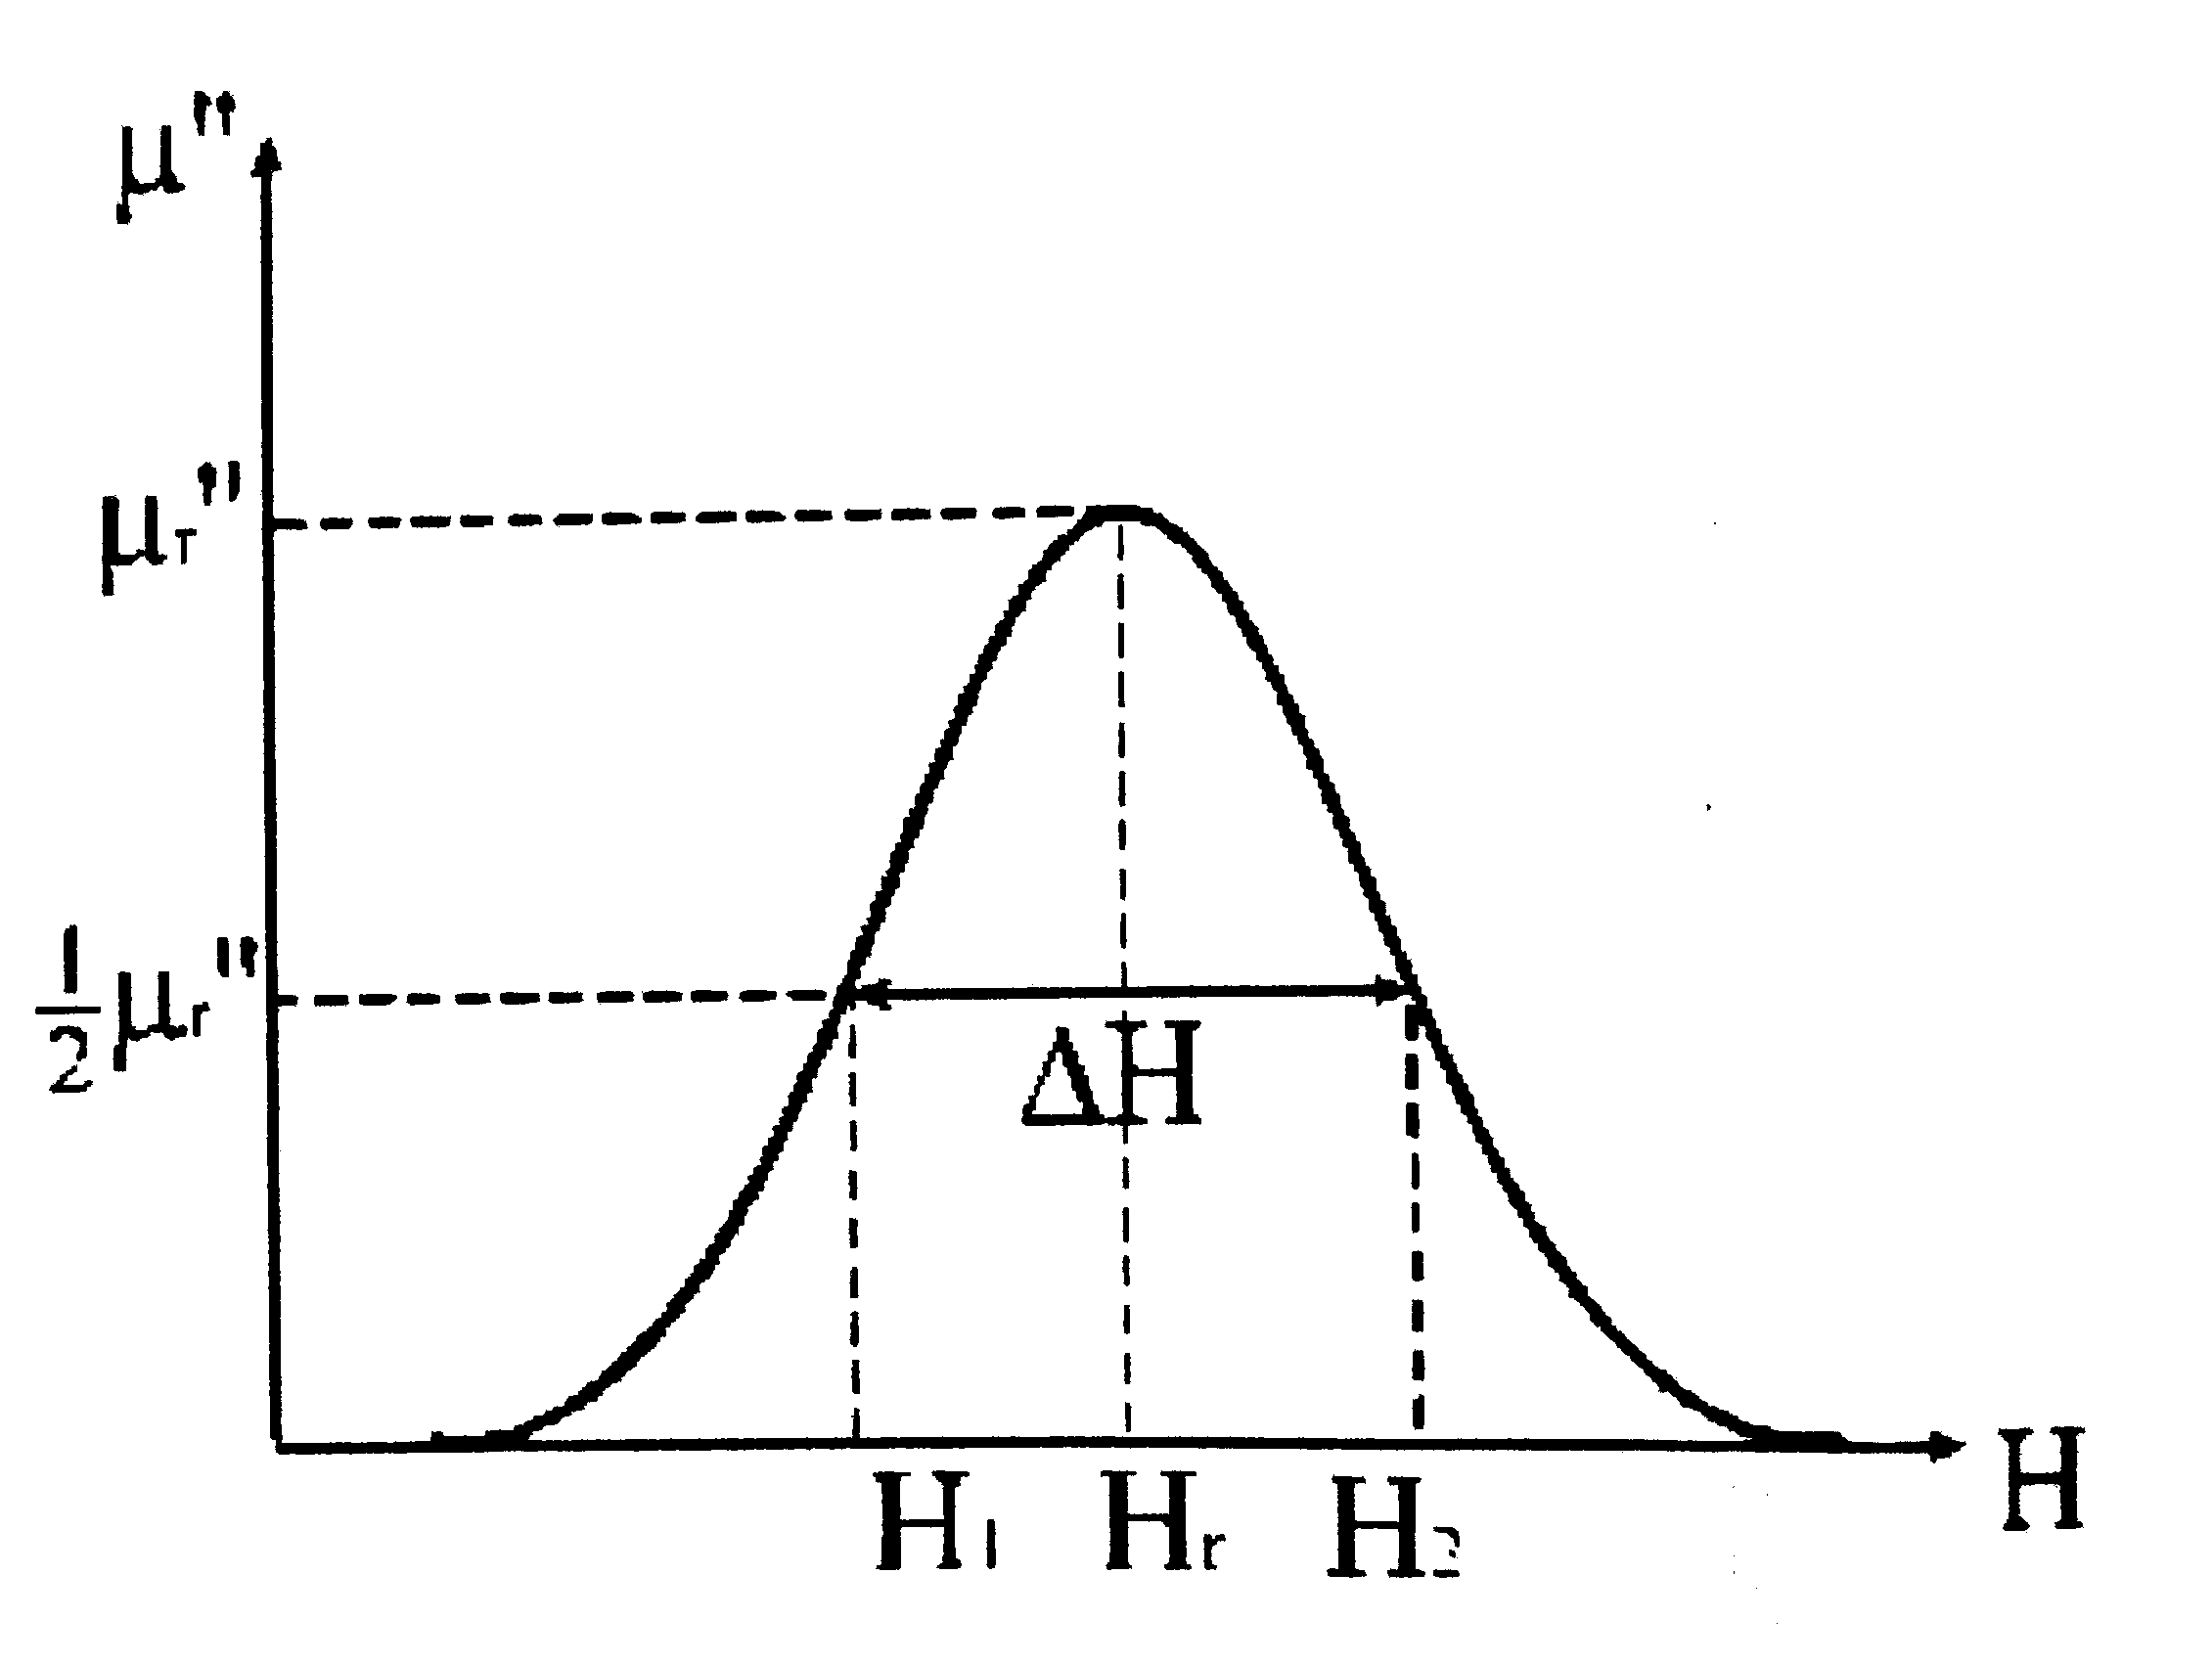
\includegraphics[height=4cm]{fig/scan/FerromagneticRessonanceCurve.png}\label{subfig:铁磁共振曲线}}\hspace{1cm}
		\subfloat[传输式谐振腔的谐振曲线]{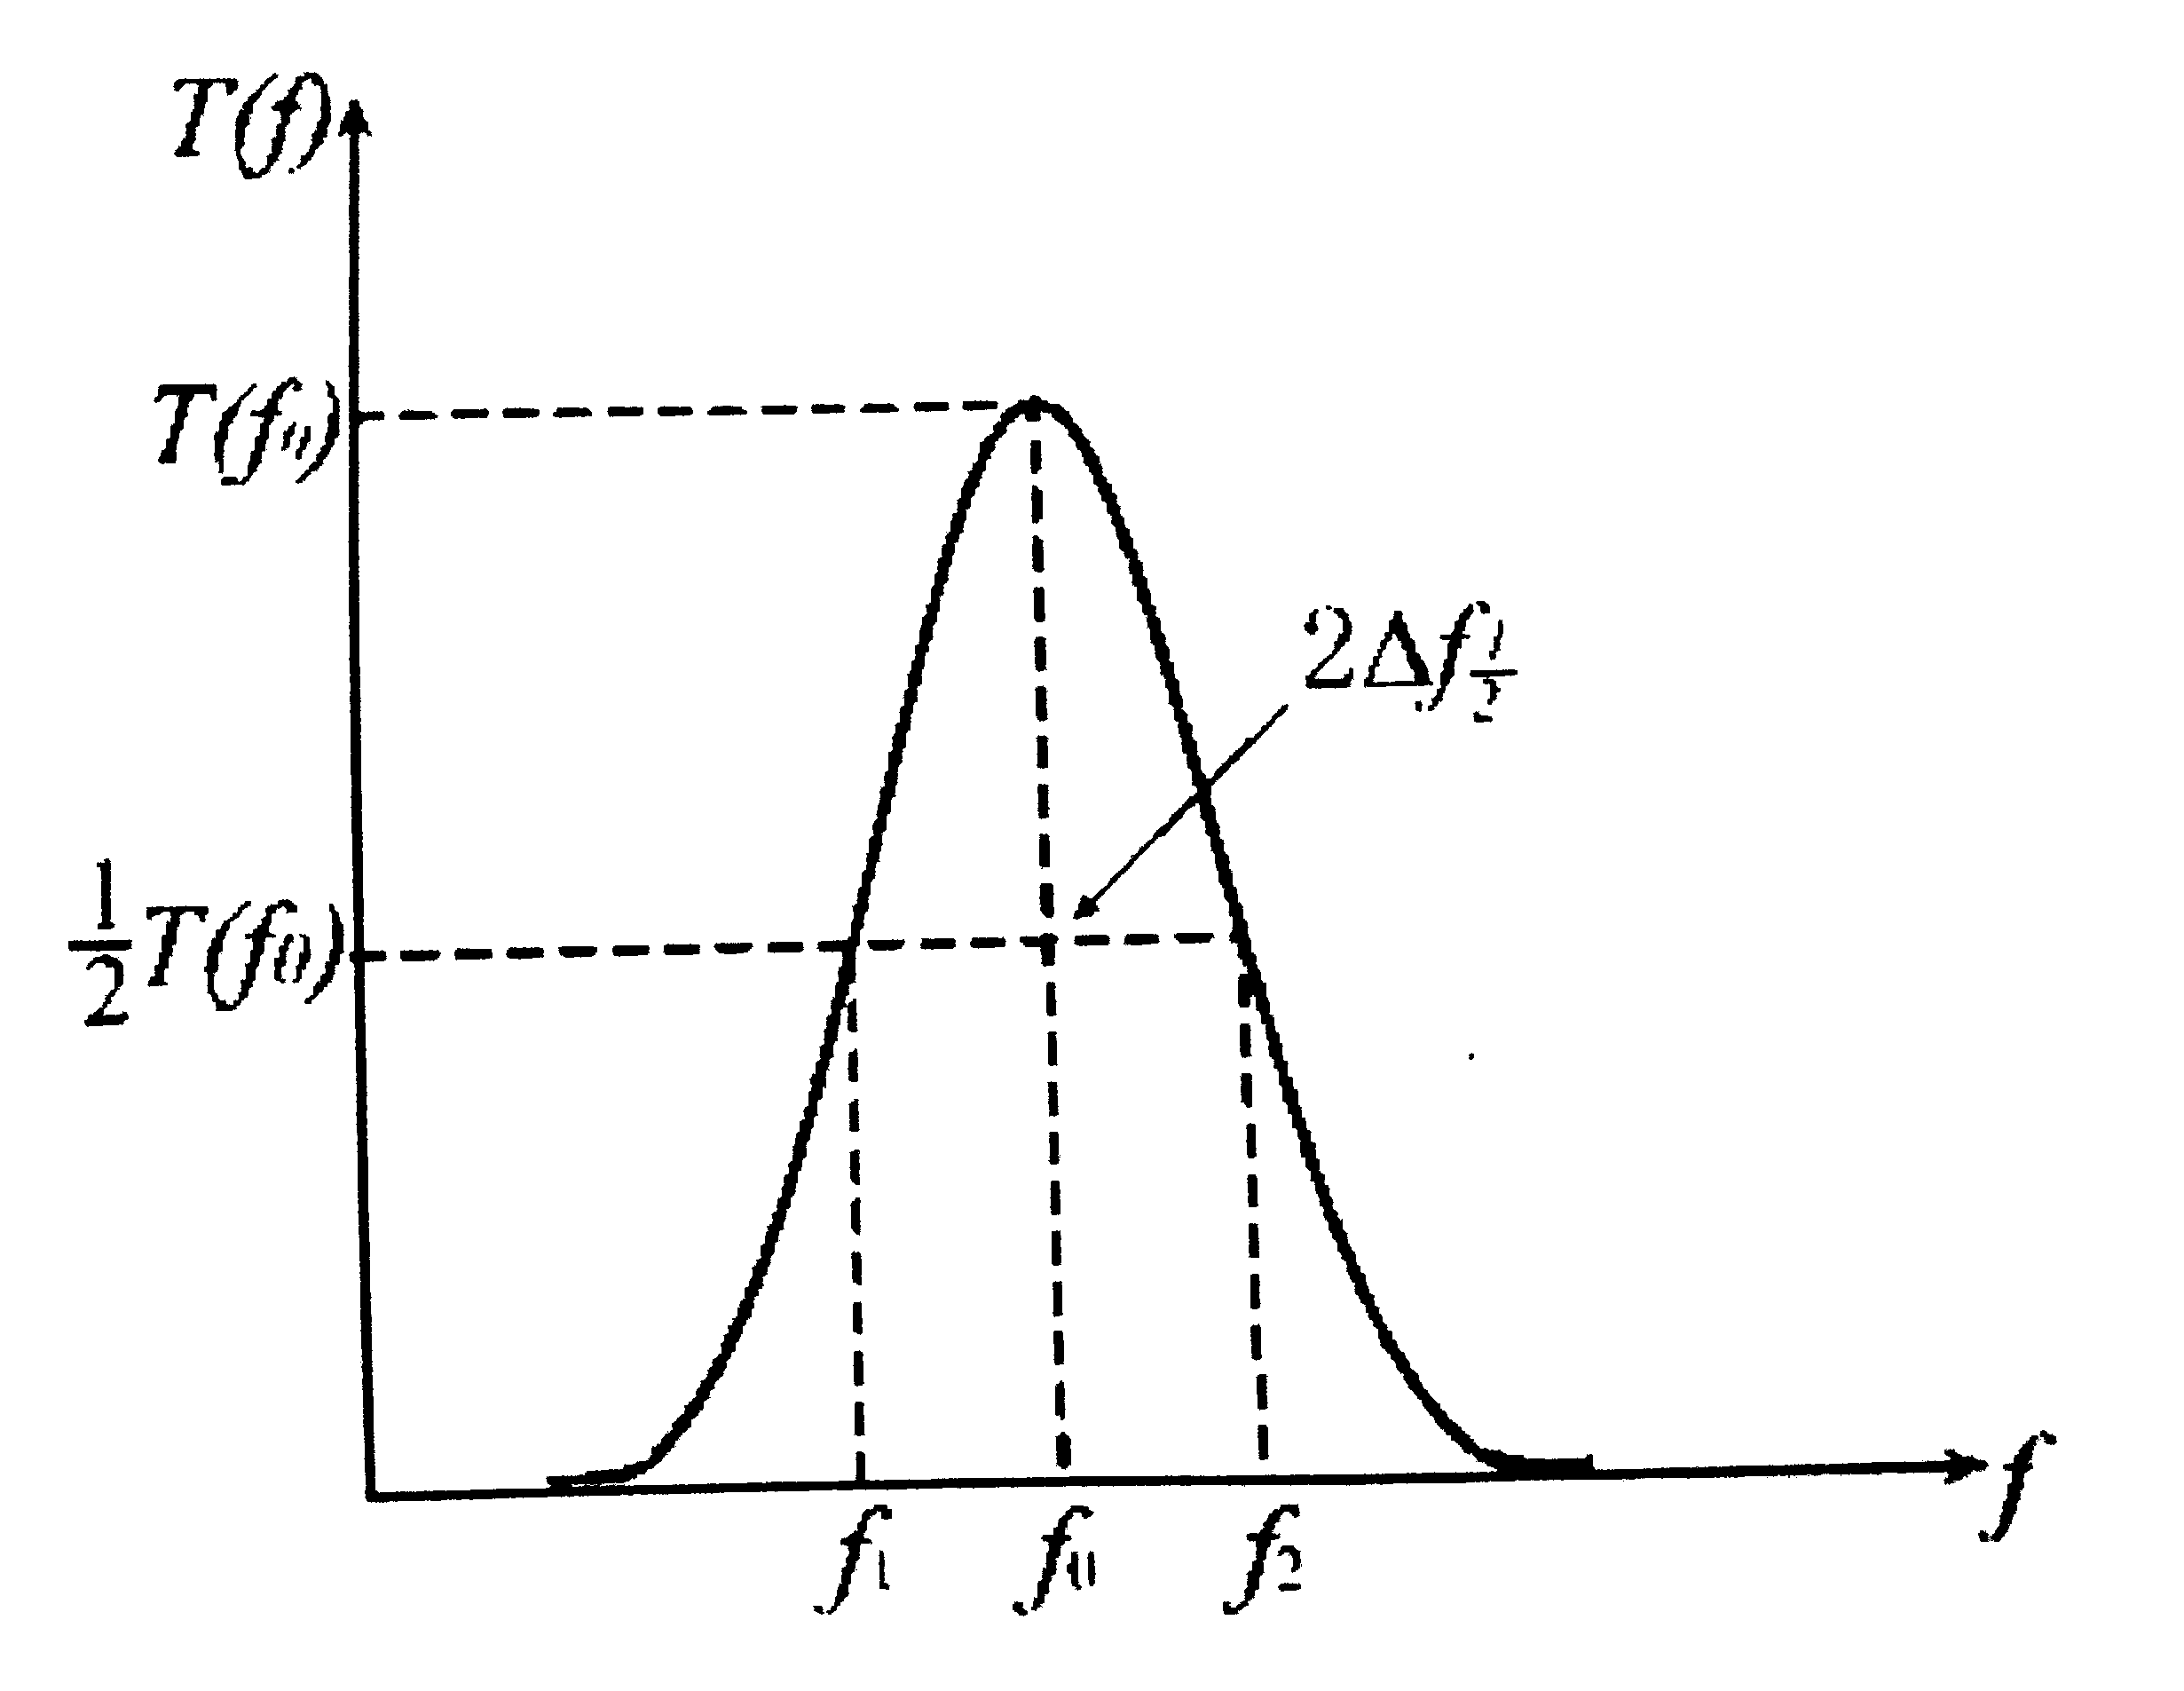
\includegraphics[height=4cm]{fig/scan/ResonatingDiagramofTransmissionresonatorFerromagneticresonanceExperiment.png}\label{subfig:传输式谐振腔的谐振曲线}}
		\caption{铁磁共振曲线和传输式谐振腔的谐振曲线}
	\end{figure}
	\subsubsection{传输式谐振腔} % (fold)
		\label{ssub:传输式谐振腔}
		\par 传输式金属谐振腔时一段矩形波导管两端加上带耦合孔的短路金属板。电磁场被导体壁局限在空腔内部连续反射;只有有合适波型和频率的电磁波能在其中形成驻波,发生谐振。
		\begin{enumerate}
			\item 谐振条件:腔长$l=p\cdot\dfrac{\lambda_g}{2},p=1,2,\cdots$;
			\item 振荡模式:本实验中的矩形波导管只传输TE$_{10}$波,腔内电磁场表示为TE$_{10p}$。$p$表示长度方向的半波数。
			\item 回路本身的品质因数$Q_0 = \omega_0\dfrac{\text{谐振时总储能}}{\text{损耗功率}}$表示谐振效率或频率选择性,即无载品质因数;加外电路后,$Q$值通常下降成为有载品质因数$Q_{\rm L}=\dfrac{Q_{0}Q_{\rm e}}{Q_{0}+Q_{\rm e}}$,其中$Q_{\rm e}$是谐振腔的外观品质因数,描述它与外电路耦合的强度。通常$Q_{\rm e}$越小时$Q_{\rm L}$也越低。
			\item 谐振曲线(传输系数-频率曲线,\cref{subfig:传输式谐振腔的谐振曲线}):$T(f)$曲线中可以得到$Q_{\rm L}=\dfrac{f_0}{|f_1-d_2|}$($f_0$表示腔的谐振频率)。
		\end{enumerate}
	% subsubsection 传输式谐振腔 (end)
	\subsubsection{用传输式谐振腔测量铁磁共振线宽} % (fold)
		\label{ssub:用传输式谐振腔测量铁磁共振线宽}
		\begin{enumerate}
			\item 谐振腔微扰公式:谐振腔中加入铁磁样品后,谐振频率受到微扰,谐振频率变化很小时,除了样品所在位置,电磁场变化都可以忽略,在TE$_{10p}$腔内,有
			\begin{equation}
				\dfrac{f-f_0}{f_0}=-A(\mu'-1),
				\quad \Delta\left(\dfrac{1}{Q_{\rm L}}\right)=2A\mu''.\label{eq:delq}
			\end{equation}
			其中$A$是与谐振腔振荡模式和体积以及样品体积相关的常量,一般满足
			\begin{equation}
				A=\dfrac{2}{1+l^2/a^2p^2}\dfrac{V_{\rm s}}{V_0}.\,(V_{\rm s}\text{是样品体积},V_0\text{是谐振腔体积})
			\end{equation}
			\item 测量方式:TE$_{10p}$腔内磁场只在$xz$平面内,外场应沿$y$方向(如\cref{subfig:测量共振线宽})。若铁氧体样品很小且放在磁场最大处,腔内保持谐振,输入功率恒定,则有
			\begin{equation}
			\begin{aligned}
				&T(f_0)=\dfrac{P_{\text{out}}(f_0)}{P_{\rm in}(f_0)}=\dfrac{4Q_{\rm L}^2}{Q_{\rm e,1}Q_{\rm e,2}}\,(Q_{\rm e,1},Q_{\rm e,2},\text{分别是输入和输出孔的外观品质因数})\\
				&\Rightarrow P_{\rm out}(f_0)=\dfrac{4P_{\rm in}(f_0)Q_{\rm L}^2}{Q_{\rm e,1}Q_{\rm e,2}}\propto Q_{\rm L}^2.
			\end{aligned}
			\end{equation}
			\begin{figure}[htbp]
				\subfloat[测量共振线宽]{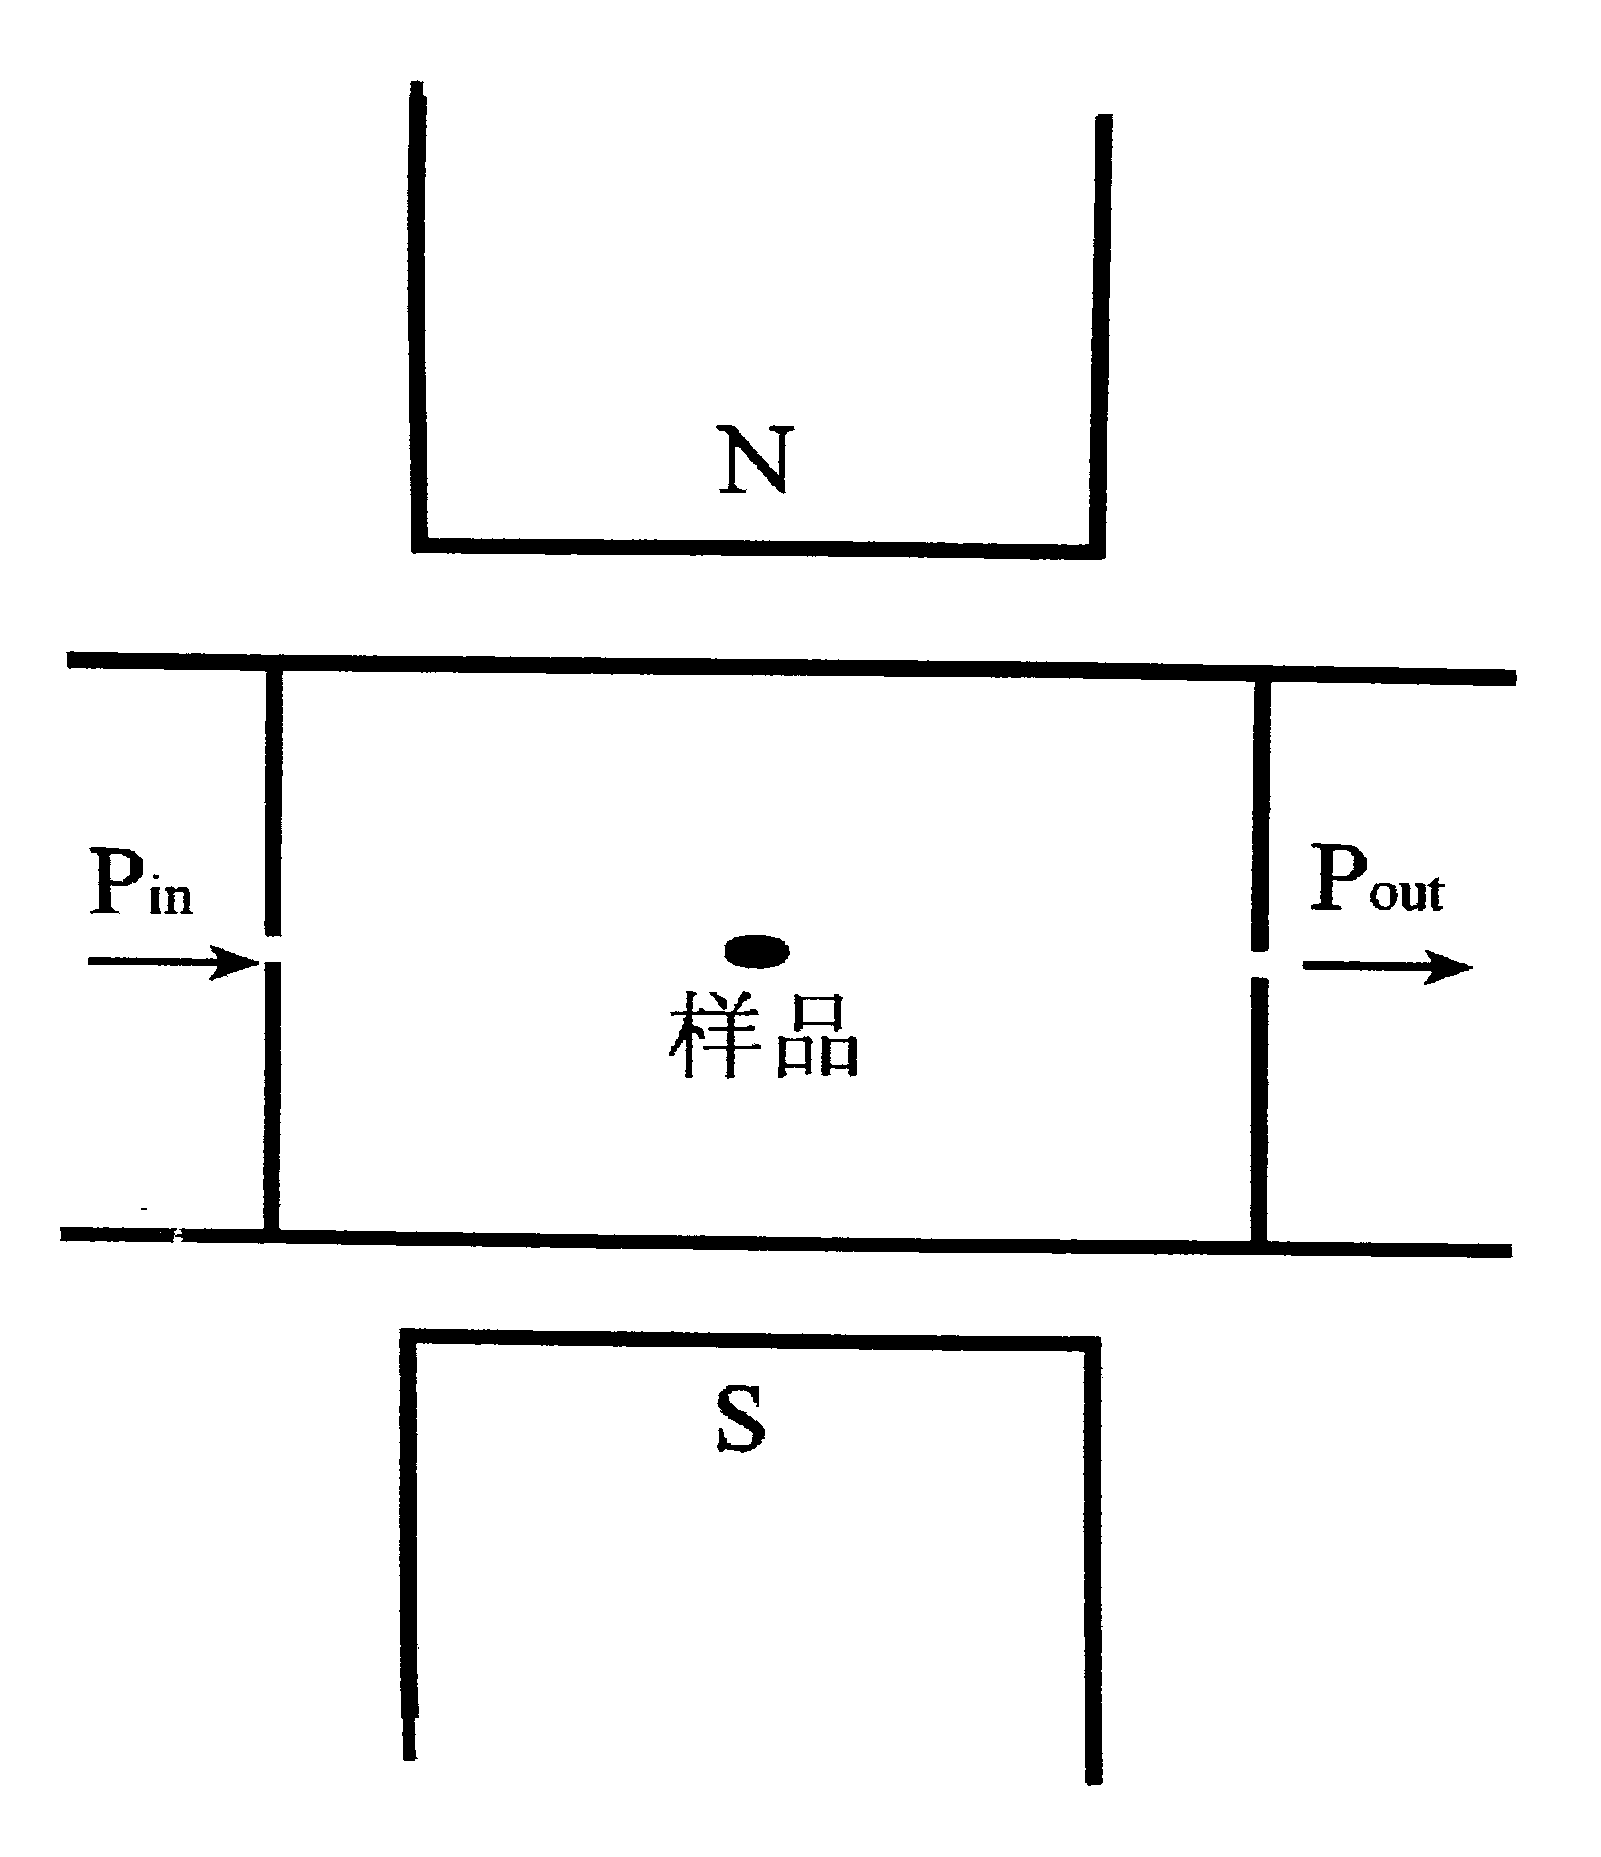
\includegraphics[height=4cm]{fig/scan/MeasuringtheresonantlinewidthofaFerromagneticSamplewithTransmissionresonatorFerromagneticresonanceExperiment.png}\label{subfig:测量共振线宽}}\hspace{2cm}
				\subfloat[$P-B$关系曲线]{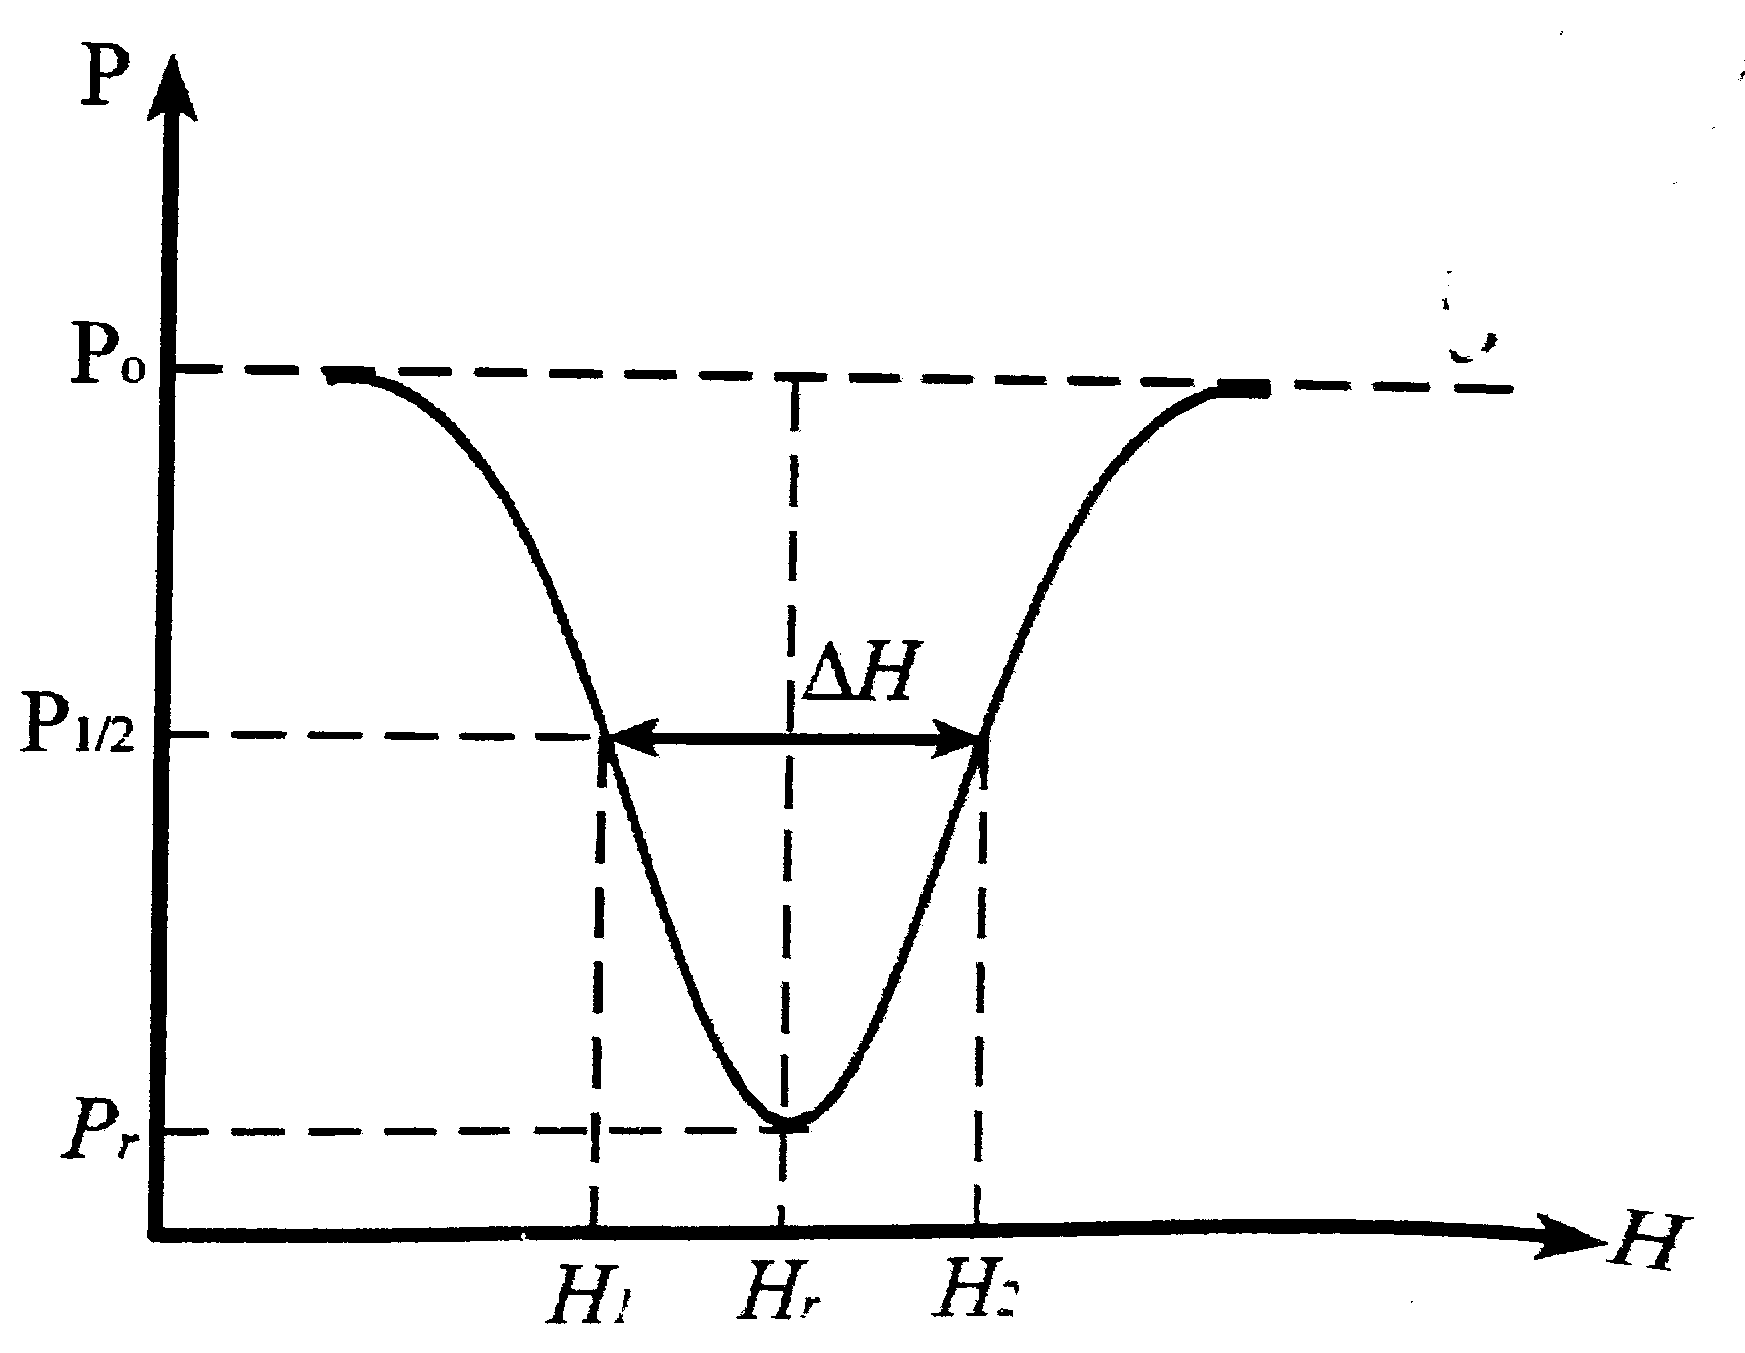
\includegraphics[height=4cm]{fig/scan/P-BDiagramofTransmissionresonatorFerromagneticresonanceExperiment.png}\label{subfig:PB关系曲线}}
				\caption{测量共振线宽和$P-B$关系曲线}
			\end{figure}
			测出上式的变化关系后就得到$Q_{\rm L}$随着$f_0$的变化,即可由\cref{eq:delq}得到$\mu''$,进而按以下方法求出$\Delta H$(\cref{subfig:PB关系曲线}):
			\par 由以上测量得出$P_{\rm out}$随着$H_0$的变化曲线,$P_0,P_{\rm r}$分别表示远离共振和共振点处的输出功率,$P_{\frac{1}{2}}$为半共振点,即$\mu''=\dfrac{\mu''_{\rm r}}{2}$的点,于是有
			\begin{equation}
				P_{\frac{1}{2}}=\dfrac{4P_0}{(1+\sqrt{P_0/P_{\rm r}})^2}.\label{eq:p}
			\end{equation}
			找到$P_{\frac{1}{2}}$对应的点就可以在图中测出$\Delta H$。
			\par $\mu$的存在会影响到谐振腔的谐振频率,即频散效应。此效应可以通过每次测量$P_{\rm out}-H_0$曲线时都重新调谐来消除。
		\end{enumerate}
	% subsubsection 用传输式谐振腔测量铁磁共振线宽 (end)
% subsection 铁磁共振 (end)